%% evaluation.tex
%%

%% ==================
\chapter{Evaluation}
\label{ch:Evaluation}
%% ==================

The results for the knapsack experiment are carefully evaluated in this section. In the first step we discuss the choice of statistical models, second we introduce \acf{NP} and the \acf{LMM} that are used to examine the recorded data, and in the last step we present the results for the parameter estimations. 

%% ===============================
\section{Choice of statistical model}
\label{ch:Evaluation:sec:StatisticalModel}
%% ===============================

In order to evaluate the data and extract statistical stress-able results, the appropriate choice of a statistical model is crucial. 
\cite{Siegel1957} defined three main criteria to identify the most suitable statistical model:
\begin{enumerate}
\item The statistical model of the test should fit the conditions of the research.
\item The measurement requirement of the test should be met by the measures used in the research.
\item From among those tests with appropriate statistical models and appropriate measurement requirements, that test should be chosen which has greatest power-efficiency\footnote{The power of a test is being defined as the probability that the test will reject the null hypothesis when in fact it is false and should be rejected \citep{Siegel1957}. Thus, a statistical test is considered to be good if it has small probability of rejecting $H_0$ when $H_0$ is true, but a large probability of rejecting $H_0$ when it is false.}.
\end{enumerate}

The conditions of the research are defined by a combination of two between-subjects and one within-subjects factors. \textit{Usergroup} and \textit{Trial} separate the treatments and the within-subjects factor \textit{Round} defines the number of observations recorded for each subject.
Table \ref{tab:OverviewVariables} gives an overview of the examined variables. All variables fulfil the measurement requirements since all dependent variables are numerical and on a scale, and all independent variables are numerical. \\
% Table generated by Excel2LaTeX from sheet 'Tabelle2'
\begin{table}
  \centering
    \begin{tabular}{l|lll}
    \toprule
    \multicolumn{1}{c|}{Independent}  & \multicolumn{3}{c}{Dependent} \\
    \midrule
    \textit{NumberOfColours} & \textit{FirstResult} & \textit{FirstTime} & \textit{DecisionTime}\\
    \textit{Round} & \textit{BestResult} & \textit{BestTime} & \textit{DecisionNumber}\\
    \textit{Trial} & \textit{FinalResult} & \textit{FinalTime}\\
    \bottomrule
    \end{tabular}%
      \caption{Overview - Independent and dependent variables}
    \label{tab:OverviewVariables}%
\end{table}%

Two statistical models are chosen to examine the data.\\
The application of \acf{NP} is aimed at answering whether or not there is an influence from the independent variables \textit{NumberOfColours}, \textit{Round} and \textit{Trial} on the dependent variables. In particular, the different filters are tested to identify the data sets that show an influence on \textit{NumberOfColours}, \textit{Round} and \textit{Trial}.\\
Subsequently, a \acf{LMM} is used to give parameter estimations to the combination of those dependent and independent variables that show an influence in the \ac{NP}s.

%%% ===============================
%\section{\acf{GLM}}
%\label{ch:Evaluation:sec:GLM}
%%% ===============================

%The implemented statistical model has two components, the structural part defines the patterns of means for each usergroup. The error model describes the variability of users within usergroup around the mean. The deviations of individual measurements are assumed to be independent.

%A \acf{GLM} is first applied to examine the hypotheses. \ac{GLM}s are considered to be powerful tests since their assumptions are very strong. Moreover, they fit the conditions of our research, since they can combine two different types of factors, between-subjects and within-subjects factors.\\
%There is one between-subjects factor, \textit{Usergroup}, that separates the treatments and one within-subjects factor, \textit{Round}, that defines the number of observations recorded for each subject.


%\afterpage{
%\begin{landscape}
%\begin{figure}[htbp] % PlotResult	
%\begin{flushleft}
%  \caption[Estimated Marginal Means over Round for each usergroup]{Estimated Marginal Means over Round for each usergroup\footnotemark}
%    \label{Estimated Marginal Means over Round for each usergroup}  
%\begin{subfigure} 
%\centering
%\includegraphics[height = 0.4\textwidth]{PlotFirstResult.pdf}
%\end{subfigure} 
%\begin{subfigure} 
%\centering
%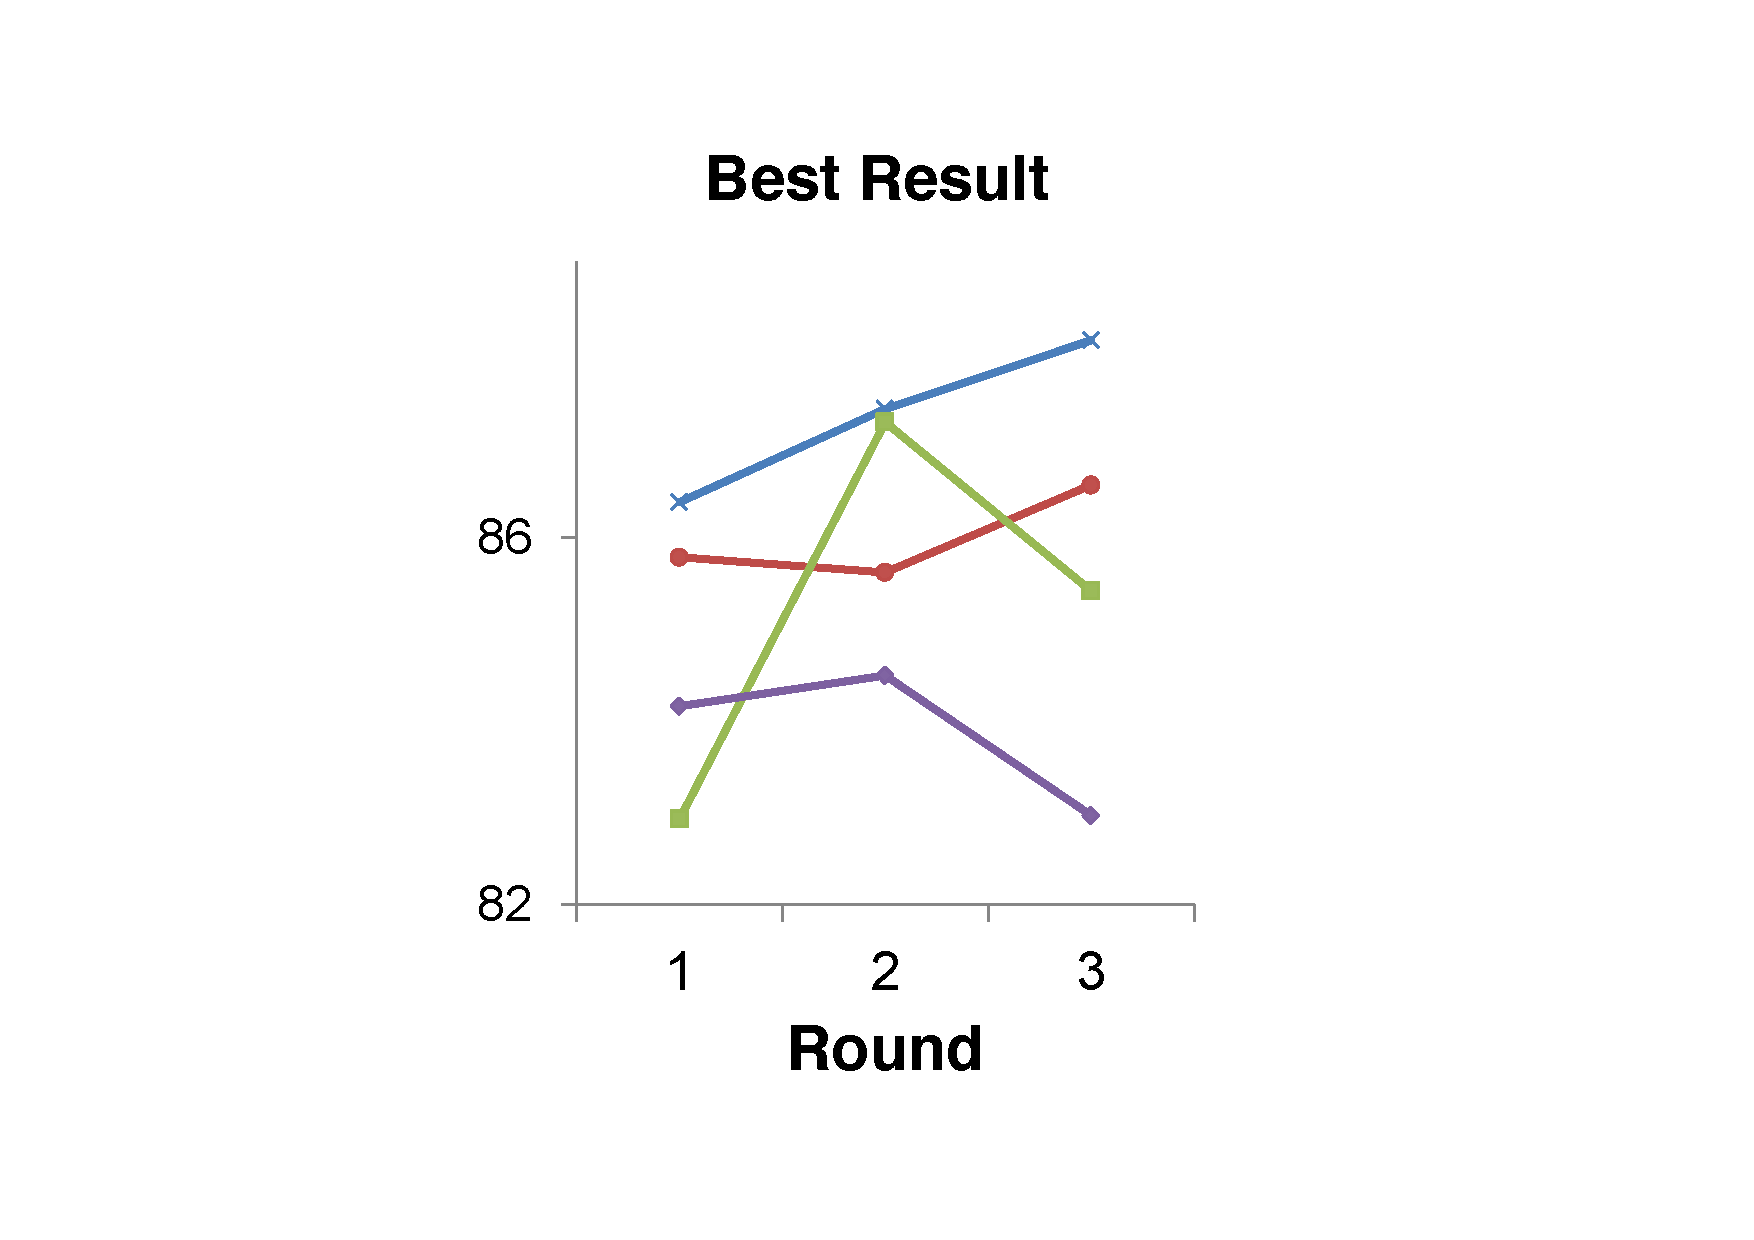
\includegraphics[height = 0.4\textwidth]{PlotBestResult.pdf}
%\end{subfigure}
%\begin{subfigure} 
%\centering
%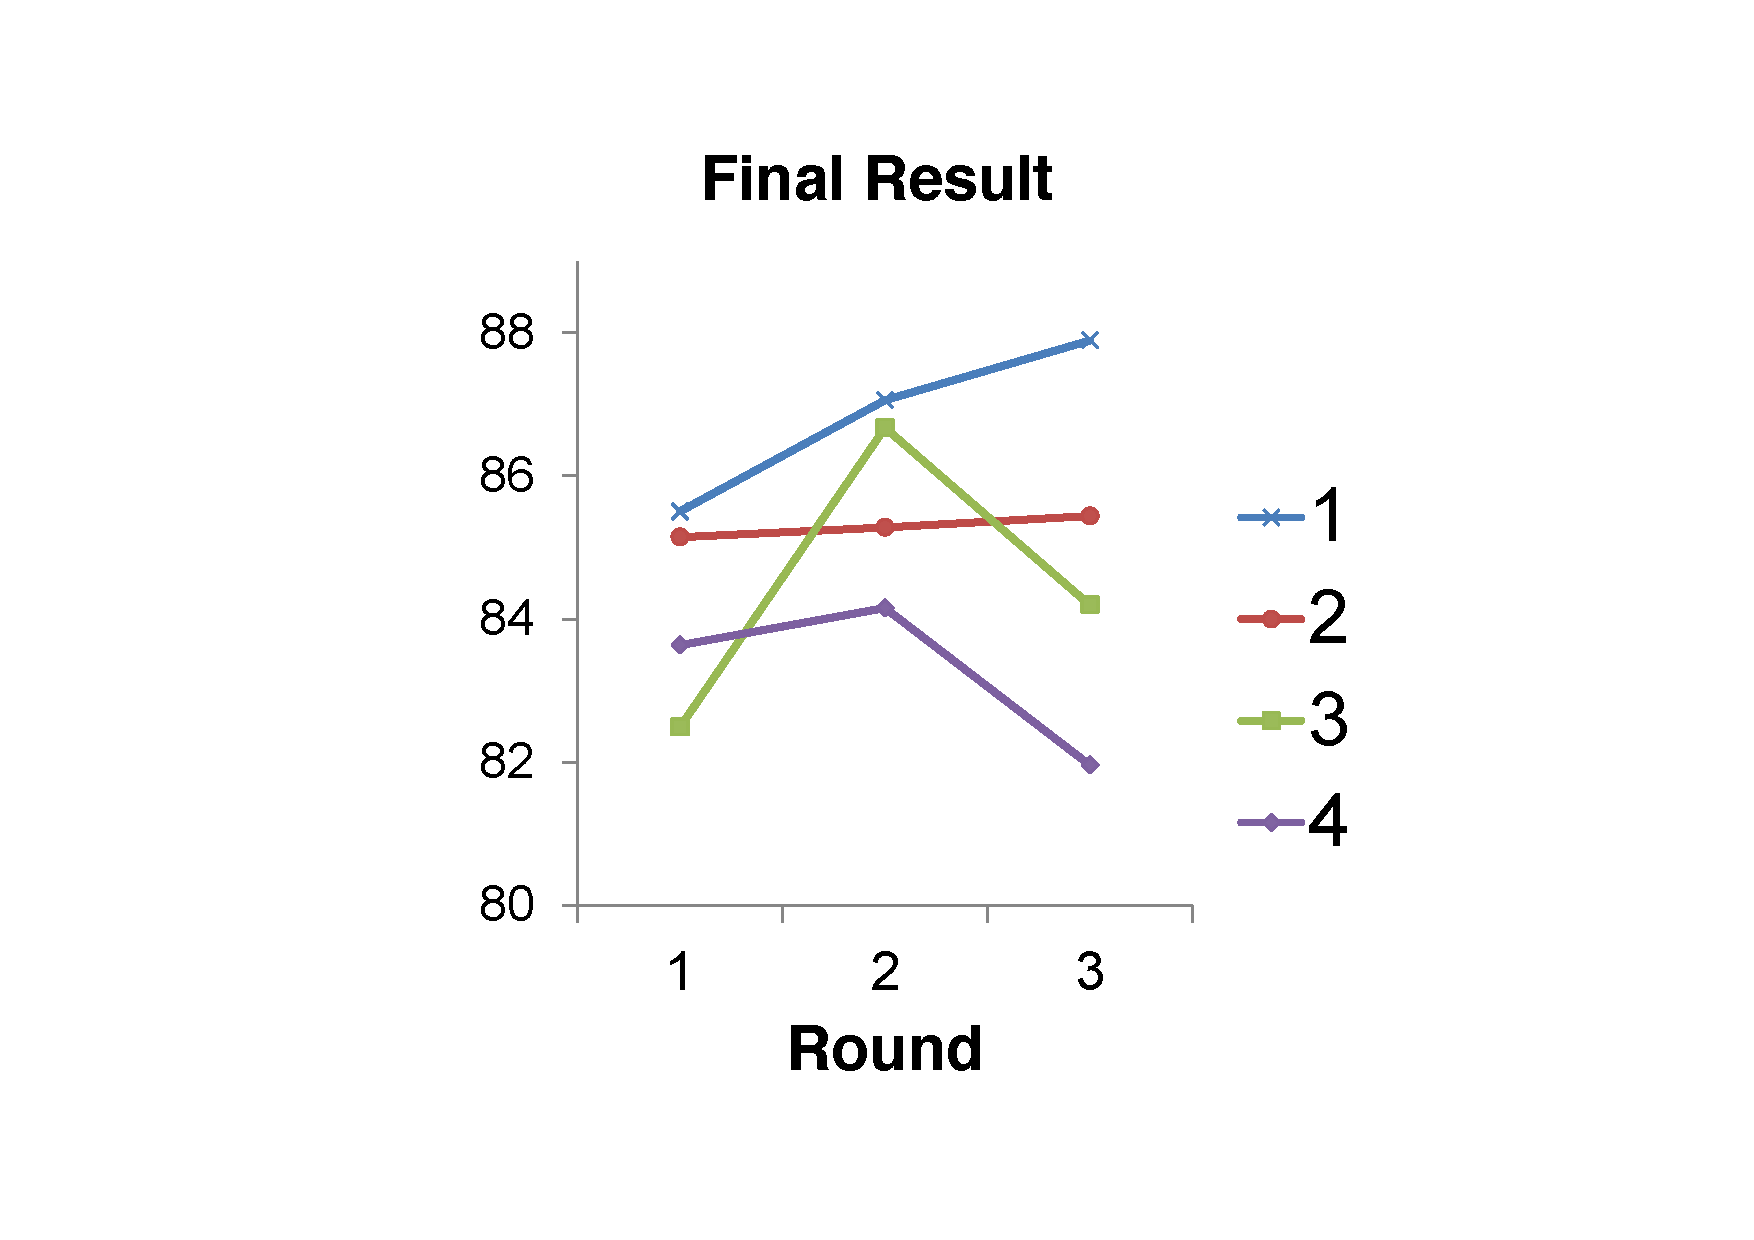
\includegraphics[height = 0.4\textwidth]{PlotFinalResult.pdf}
%\end{subfigure}
% \line(1,0){600}
%
%\begin{subfigure} 
%\centering
%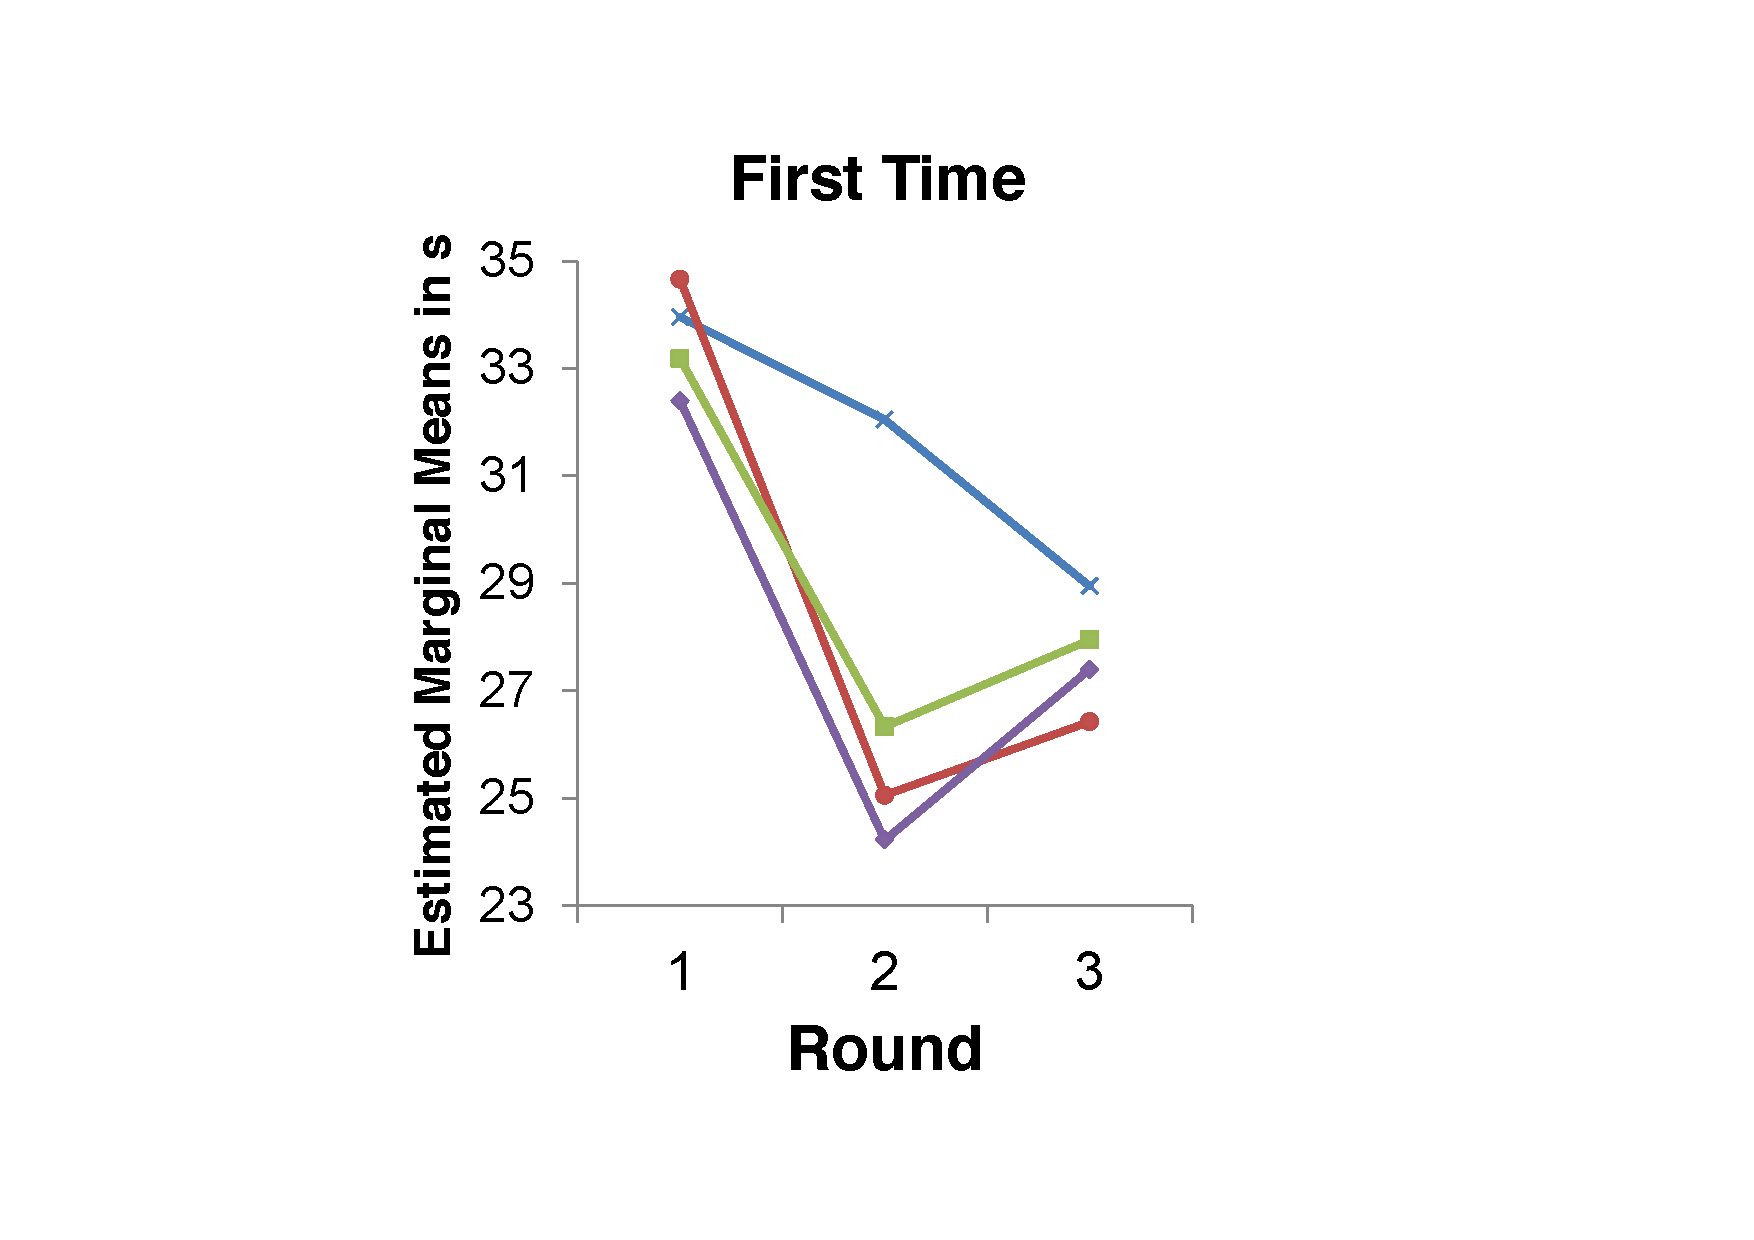
\includegraphics[height = 0.4\textwidth]{PlotFirstTime.pdf}
%\end{subfigure} 
%\begin{subfigure} 
%\centering
%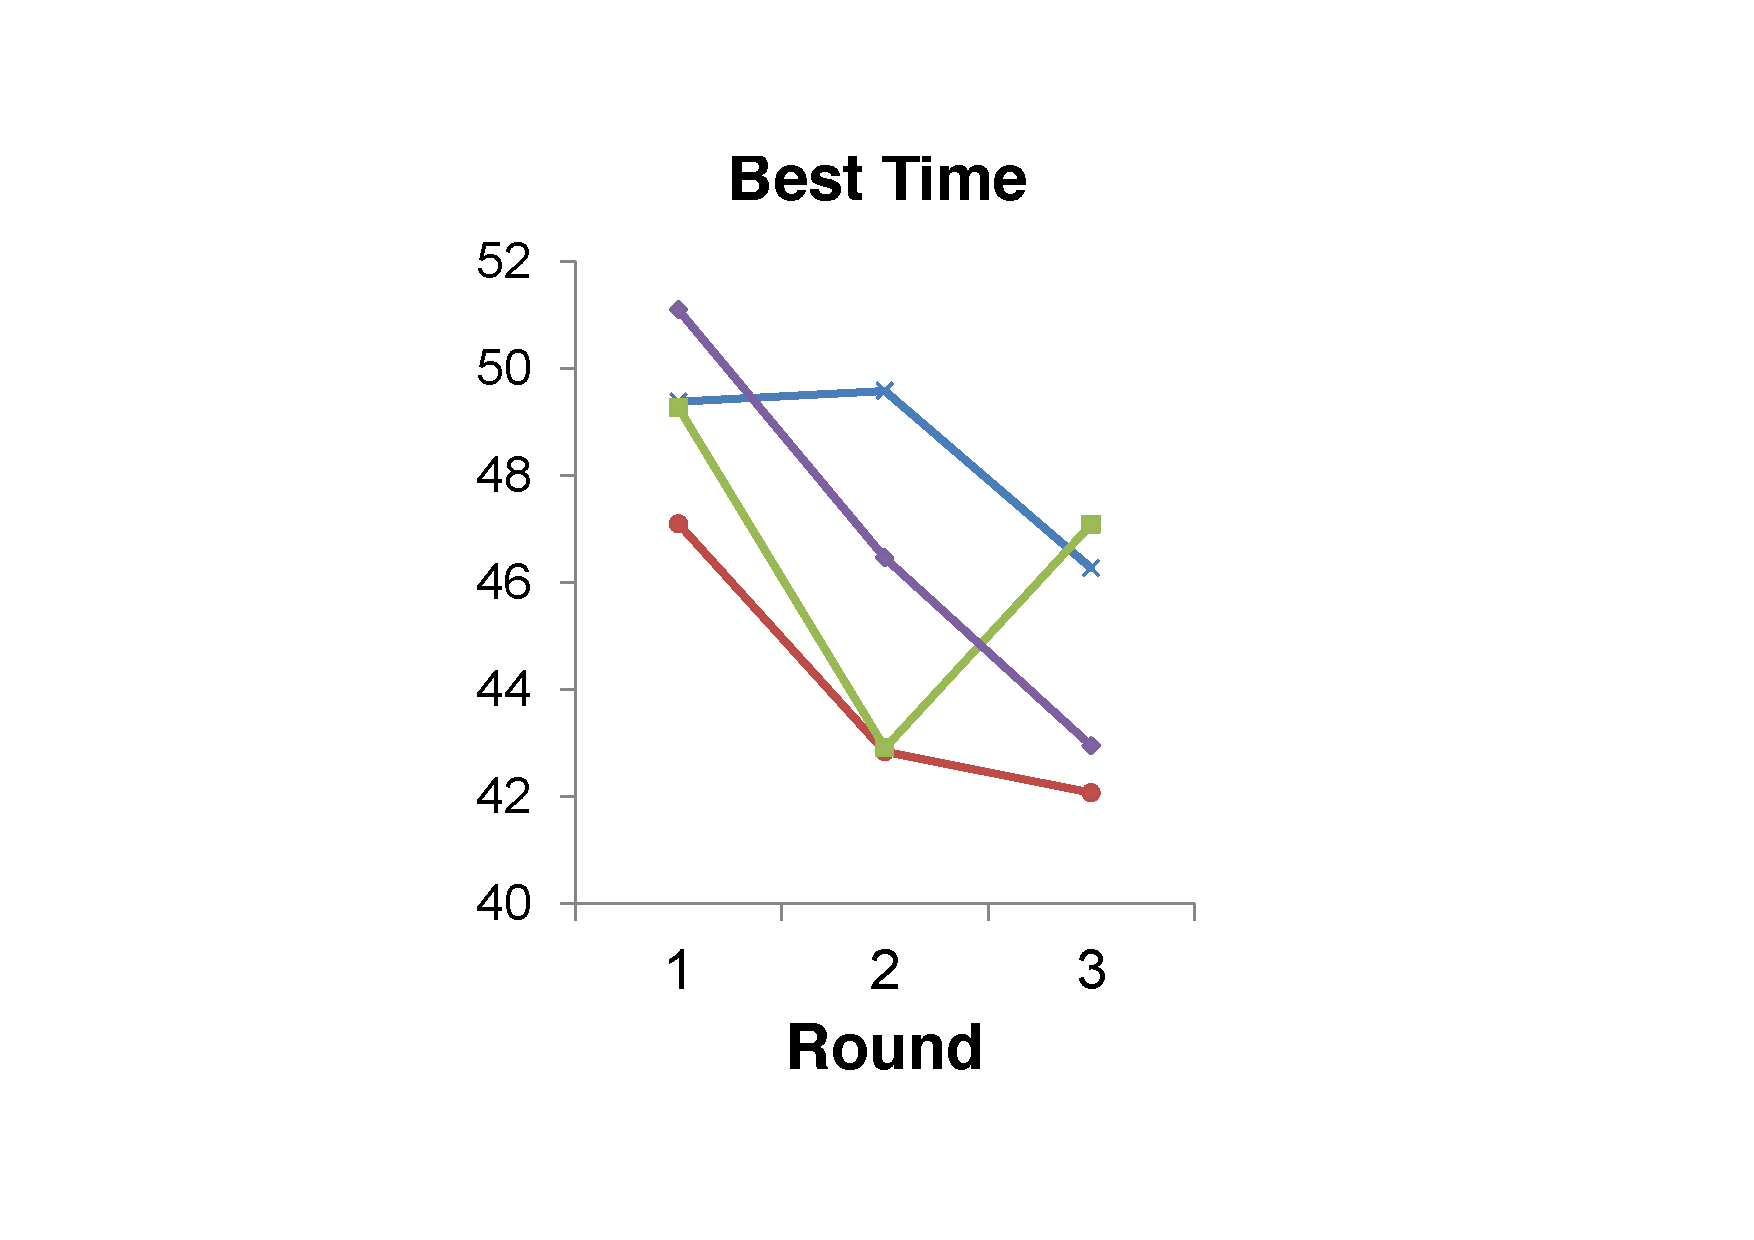
\includegraphics[height = 0.4\textwidth]{PlotBestTime.pdf}
%\end{subfigure}
%\begin{subfigure} 
%\centering
%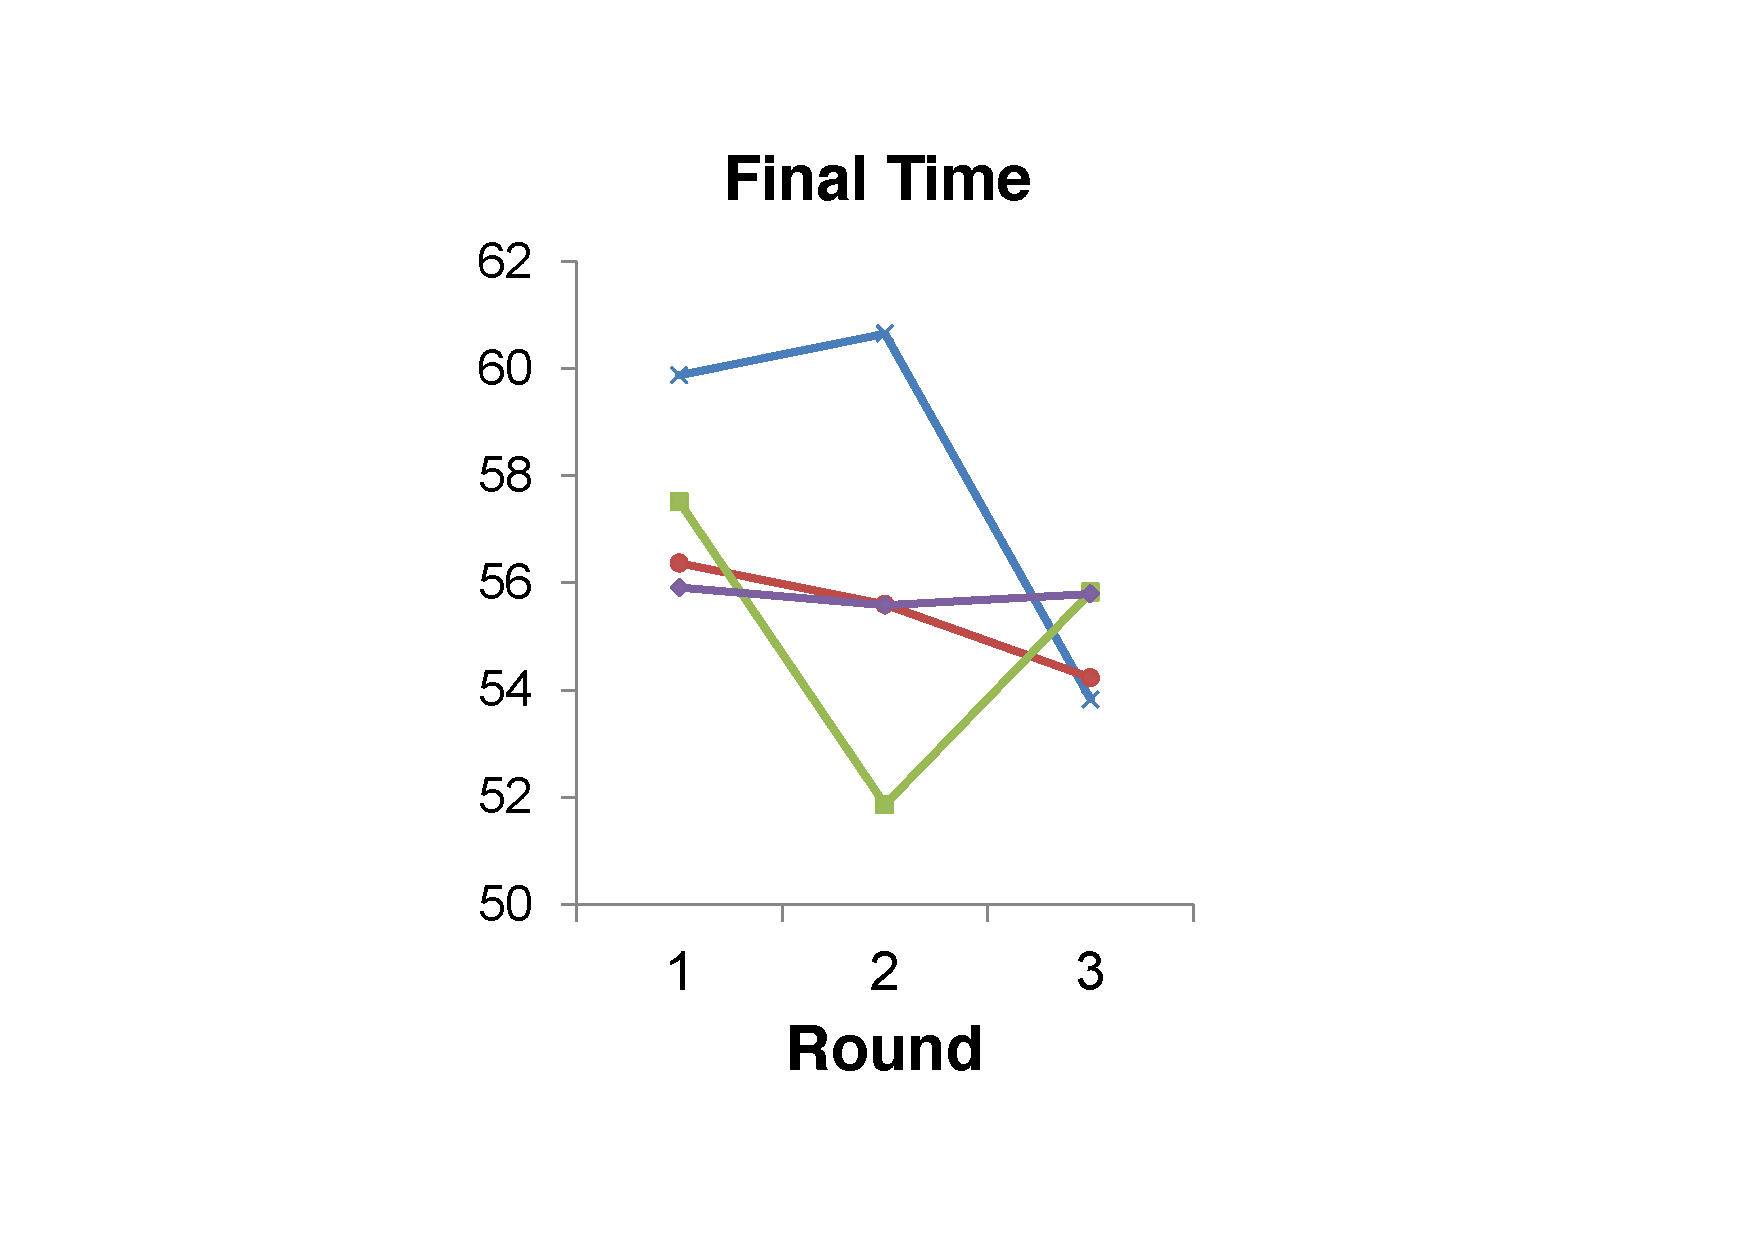
\includegraphics[height = 0.4\textwidth]{PlotFinalTime.pdf}
%\end{subfigure}
%\begin{subfigure} 
%\centering
%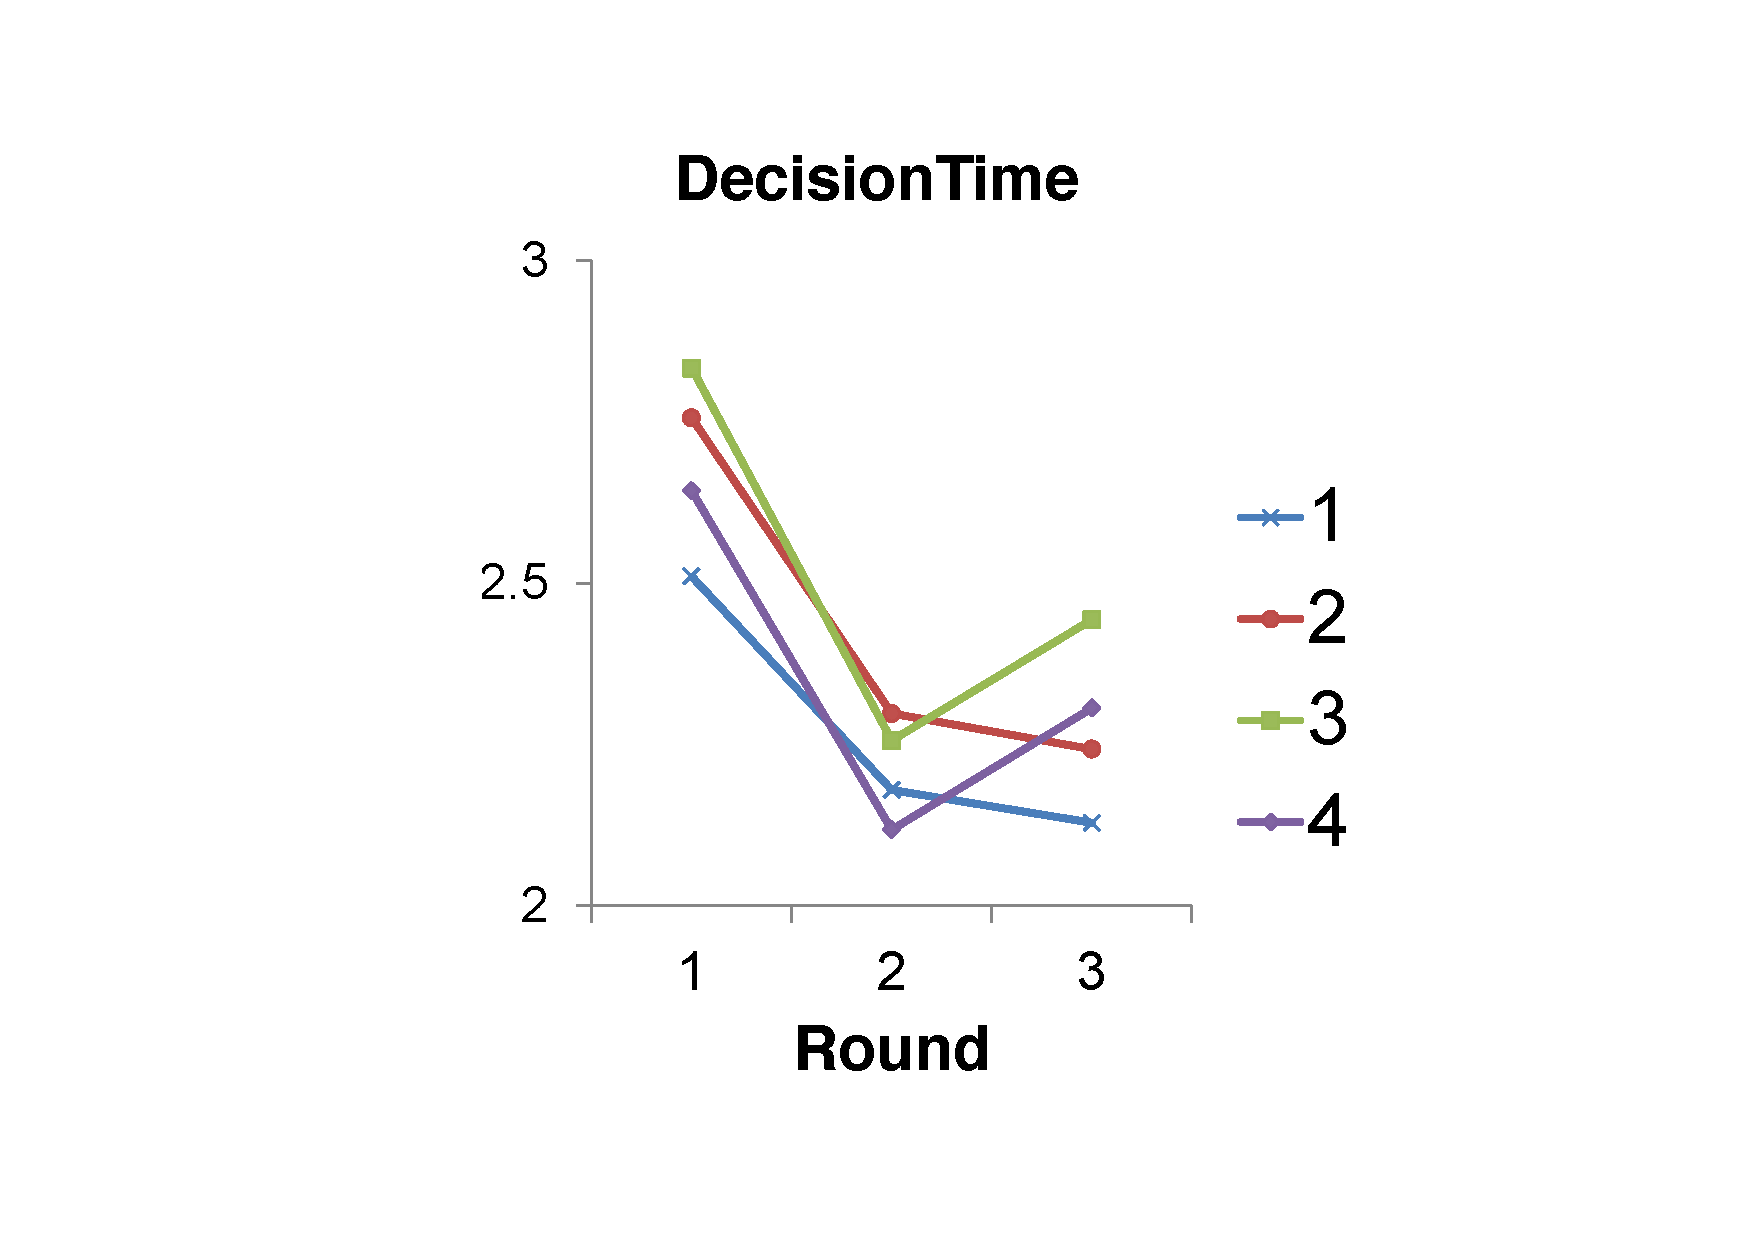
\includegraphics[height = 0.4\textwidth]{PlotDecisionTime.pdf}
%\end{subfigure} 
%\end{flushleft}
%\end{figure}
%\end{landscape}
%}
%\footnotetext{The values for the estimated marginal means are transformed back into the original scale.}
%\subsection{Tests of Between-Subjects Effects: \textit{Usergroup}}
%The estimated marginal means from the \ac{GLM} are displayed in Figure \ref{Estimated Marginal Means over Round for each usergroup}.\\
%For the three results types, Figure \ref{Estimated Marginal Means over Round for each usergroup} shows a clear difference in the results between usergroups 1 and 4, yet usergroups 2 and 3 return mixed results and therefore dilute the validity of the model. For \textit{FirstTime}, usergroups 2, 3 and 4 have very similar values, the variable \textit{BestTime} is noticeable different for usergroup 1 and 2. Usergroups 2 and 3 show similar values for \textit{FinalTime}, the pairs of usergroup 1 and 2, and 3 and 4 have similar trends for \textit{DecisionTime}.\\
%The significance values for the influence of the variable \textit{Usergroup} (Tabel \ref{tab:GLMUsergroup}) do not confirm a general influence on all usergroups, since they are much greater than .05. This leads to the conclusion that the number of colours does not contribute to the model using all usergroups.\\
% If usergroups 2 and 3 are excluded from the data, the influence of \textit{Usergroup} gets significant on the .10 value for all result types. Nevertheless the partial $\eta^2$ remains low. All time variables are not significantly influenced by the usergroups.
%% Table generated by Excel2LaTeX from sheet 'Usergroup'
%\begin{table}[htbp]
%  \centering
%  \caption{GLM - Results for \textit{Usergroup} effect}
%    \label{tab:GLMUsergroup}
%    \begin{tabular}{c||c|c||c|c}
%    \multirow{2}[1]{*}{Variable} & \multicolumn{2}{c||}{No Filter} & \multicolumn{2}{c}{Usergroup 1 and 4} \\
%          & p     & $\eta_{partial}^2$ & p & $\eta_{partial}^2$ \bigstrut[b]\\
%    \hline
%    \textit{First Result} & ns    & -   & $\cdot$    & .04 \bigstrut\\
%    \hline
%    \textit{BestResult} & ns    & -   & $\cdot$     & .03 \bigstrut\\
%    \hline
%    \textit{FinalResult} & ns    &  -  & $\cdot$     & .03 \bigstrut\\
%    \hline
%    \multicolumn{5}{c}{\textit{ns: FirstTime, BestTime, FinalTime, DecisionTime}} \bigstrut[t]\\
%    \end{tabular}%
%\end{table}%
%		
%\subsection{Tests of Within-Subjects Effects: \textit{Round}}
%As indicated by Figure \ref{Estimated Marginal Means over Round for each usergroup}, the \textit{Round} influence seems to be positive for usergroup 1, yet usergroups 2, 3 and 4 do not return distinct results. No overall monotonous effect from \textit{Round} on the times can be detected in the graphs, however there seems to be a noticeable influence from round 1 to 2 on \textit{FirstTime}, \textit{BestTime} and \textit{DecisionTime}.
%
%A Univariate Test, using the Greenhouse-Geisser, Huynh-Feldt and Lower-bound tests\footnote{The Sphericity Assumed
%test is not included since the covariance matrix assumption is not met.}, confirms that for \textit{BestResult}, \textit{FinalResult}, \textit{FirstTime}, \textit{BestTime} and \textit{DecisionTime} the within-subjects effects contribute to the model (Tabel \ref{tab:GLMRound}). No significant results are found for the \textit{FirstResult} and \textit{FinalTime}. Nevertheless the values for the $\eta_{partial}^2$ are very small (< .1), so the \textit{Round} effect only explains a small portion of the variation in the outcome of the majority of the variables. The $\eta_{partial}^2$ for \textit{DecisionTime},however, has a higher value.
%% Table generated by Excel2LaTeX from sheet 'Round'
%\begin{table}[htbp]
%  \centering
%  \caption[GLM - Results for Round effect]{GLM - Results for \textit{Round} effect\footnotemark}
%    \label{tab:GLMRound}
%    \begin{tabular}{c|c|c|c|c|c|c}
%    \multirow{2}[1]{*}{Variable} & \multicolumn{2}{c|}{No Filter} & \multicolumn{2}{c|}{Usergroup 1 \& 4} & \multicolumn{2}{c}{Round 1 \& 2} \\
%          & p     & $\eta_{partial}^2$ & p     & $\eta_{partial}^2$ & p     & $\eta_{partial}^2$ \bigstrut[b]\\
%    \hline
%    \textit{BestResult} & $\cdot$     & .02 & ns    & -     & *    & .03 \bigstrut[t]\\
%    \hline
%    \textit{FinalResult} & $\cdot$     & .02 & ns    & -     & *    & .03 \bigstrut[b]\\
%    \hline
%    \textit{FirstTime} & *    & .08   & *    & .05   & **   & .13 \bigstrut\\
%    \hline
%    \textit{BestTime} & *    & .03   & $\cdot$     & .03   & *    & .03 \bigstrut\\
%    \hline
%    \textit{DecisionTime} & *    & .19   & **   & .16   & **   & .27 \bigstrut[t]\\
%    \multicolumn{7}{c}{\textit{ns: FirstResult, FinalTime}} \\
%    \end{tabular}%
%\end{table}%
%\footnotetext{Greenhouse-Geisser, Huynh-Feldt, Lower-bound statistics aggregated.}
%
%The graphical assumption for usergroup 1 - a potential influence from \textit{Round} on the three result types - is not acknowledged by the results from the tests. Looking at the specific \textit{Round} level, the contrast results indicate that the \textit{Round} influence is significant for the 1\textsuperscript{st} to the 2\textsuperscript{nd} round for all the displayed variables in the table (p < .05).\\
%%% Table generated by Excel2LaTeX from sheet 'Latex'
%%\begin{table}[htbp]
%%  \centering
%%  \caption[GLM - Results for the different effects]{\ac{GLM} - Results for the different effects\footnotemark}
%%    \label{GLM - Results for the different effects}%
%%    \begin{tabular}{c|c||c|c||c|c||c|c}
%%    \multirow{2}[1]{*}{Effect} & \multirow{2}[1]{*}{Variable} & \multicolumn{2}{c||}{No Filter} & \multicolumn{2}{c||}{Usergroup 1 \& 4} & \multicolumn{2}{c}{Round 1 \& 2} \\
%%          &       & p     & partial $\eta^2$ & p     & partial $\eta^2$ & p     & partial $\eta^2$ \bigstrut[b]\\
%%    \hline
%%    \multirow{3}[6]{*}{Usergroup} & \textit{FirstResult} & .41  & .02  & \cellcolor{darkgrey}.04  & \cellcolor{grey}.04  & -     & - \bigstrut\\
%%\cline{2-8}          & \textit{BestResult} & .58  & .01  & \cellcolor{darkgrey}.10  & \cellcolor{grey}.03  & -     & - \bigstrut\\
%%\cline{2-8}          & \textit{FinalResult} & .56  & .01  & \cellcolor{darkgrey}.10  & \cellcolor{grey}.03  & -     & - \bigstrut\\
%%    \hline
%%    \multirow{3}[6]{*}{Round\footnotemark} & \textit{FirstResult} & >  .5 & < .01 & >  .9 & < .01 & >  .9  & < .01 \bigstrut\\
%%\cline{2-8}          & \textit{BestResult} & \cellcolor{darkgrey}<  .1 & < \cellcolor{grey}.02 & >  .6 & < .01 & \cellcolor{darkgrey}.03  & \cellcolor{grey}.03 \bigstrut\\
%%\cline{2-8}          & FinalResult & \cellcolor{darkgrey}<  .1 & \cellcolor{grey}< .02 & >  .3 & < .01 & \cellcolor{darkgrey}.01  & \cellcolor{grey}.03 \bigstrut\\
%%    \hline
%%    Usergroup & \textit{FirstResult} & >  .2 & < .01 & .14  & .02  & \cellcolor{darkgrey}.04  & \cellcolor{grey}.05 \bigstrut\\
%%\cline{2-8}    *     & \textit{BestResult} & \cellcolor{darkgrey}<  .1 & \cellcolor{grey}< .02 & .59  & < .01  & \cellcolor{darkgrey}.06  & \cellcolor{grey}.04 \bigstrut\\
%%\cline{2-8}    Round\footnotemark & \textit{FinalResult} & \cellcolor{darkgrey}<  .1 & \cellcolor{grey}< .03 & .46  & .01  & .14  & .03 \bigstrut[t]\\
%%    \end{tabular}%
%%\end{table}%
%%\footnotetext{Significance level is .10. Cases with rejected hypothesis are marked in dark grey, the corresponding partial $\eta^2$ in grey.}
%%\footnotetext{Greenhouse-Geisser, Huynh-Feldt, Lower-bound statistics aggregated.}
%
%\subsection{Tests of a combination of Within-Subjects Effects and Between-Subjects Effects}
%The univariate test combining the contribution of \textit{Usergroup} and \textit{Round} indicates a minor influence of the combined variables on \textit{BestResult} and \textit{FinalResult} with all statistics showing significant values on the .10 level (Table \ref{tab:GLMUsergroupRound}). This is most likely caused by the significant individual influence from \textit{Round}.
%On the specific \textit{Round} level, however, one can also find a significant contribution from Round 1 to Round 2 on the \textit{FirstResult}, yet the $\eta_{partial}^2$ is again very low. These findings are rather suspect, since there is no significant influence from each individual variable detectable for the \textit{FirstResult}.
%For the time variables, no significant influence by a combination between \textit{Usergroup} and \textit{Round} can be detected.
%% Table generated by Excel2LaTeX from sheet 'UsergroupRound'
%\begin{table}[htbp]
%  \centering
%  \caption[GLM - Results for Usergroup \& Round effect]{GLM - Results for \textit{Usergroup} \& \textit{Round} effect\footnotemark}
%    \label{tab:GLMUsergroupRound}
%    \begin{tabular}{c||c|c||c|c||c|c}
%    \multirow{2}[1]{*}{Variable} & \multicolumn{2}{c||}{No Filter} & \multicolumn{2}{c||}{Usergroup 1 \& 4} & \multicolumn{2}{c}{Round 1 \& 2} \\
%          & p     & $\eta_{partial}^2$ & p     & $\eta_{partial}^2$ & p     & $\eta_{partial}^2$ \bigstrut[b]\\
%    \hline
%    \textit{First Result} & ns    & -     & ns    & .02   & *    & .05 \bigstrut\\
%    \hline
%    \textit{BestResult} & $\cdot$     & .02   & ns    & .00   & $\cdot$     & .04 \bigstrut\\
%    \hline
%    \textit{FinalResult} & $\cdot$     & .03   & ns    & .01   & ns    & - \bigstrut[t]\\
%    \multicolumn{7}{c}{\textit{ns: FirstTime, BestTime, FinalTime, DecisionTime}} \\
%    \end{tabular}%
%\end{table}%
%\footnotetext{Greenhouse-Geisser, Huynh-Feldt, Lower-bound statistics aggregated.}
%
%We conclude that even tough the tests partly return significant values for the mutual influence by \textit{Usergroup} and \textit{Round}, these variables only explain a small portion of the values for the result types, since the partial $\eta_{partial}^2$ is very low.
%
%% ===============================
\section{\acf{NP}}
\label{ch:Evaluation:sec:Non-parametrictest}
%% ===============================

\acl{NP} are statistical models that do not specify restrictive conditions \citep{Siegel1957}. As a result, \ac{NP} only make minimal assumptions regarding the underlying distribution of the data, so they do not require the data to be normally distributed. Furthermore, the tests rank the values instead of looking at the values themselves which makes them robust against outliers.\\
Two different categories of tests are used; an independent-samples test, analysing the dependent variables that are grouped by \textit{NumberOfColours} and \textit{Trial}; and a test for related samples, comparing \textit{Rounds} for the same set of users. 

\subsection{Tests of Independent samples: \textit{NumberOfColours} \& \textit{Trial}}
Two tests are conducted for the independent samples. The Kruskal-Wallis Test of Independent Samples\footnote{For the SPSS source code of the two tests, refer to this \href{http://publib.boulder.ibm.com/infocenter/spssstat/v20r0m0/topic/com.ibm.spss.statistics.help/alg_nonparametric_independent_wald-wolfowitz.htm}{Link}.}, comparing the distributions per \textit{NumberOfColours}, as well as the Mann-Whitney Test, which compares the two \textit{Trials} against each other.\\
Null and alternative hypotheses are defined in the following way: 

\textbf{Kruskal-Wallis- \& Mann-Whitney-Test} \\
\textbf{H\textsubscript{0}:} \textit{The distribution of the dependent variables are the same across different usergroups.}\\
\textbf{H\textsubscript{A}:} \textit{At least one distribution is different.}

\paragraph{\textit{Trial}}
The Mann-Whitney-Test retains the null hypothesis for all dependent variables for the influence of \textit{Trial} (Table \ref{NPTest}), so the different bonus systems do not seem to have an influence on the data.

\paragraph{\textit{NumberOfColours}}
The results for the Kruskal-Wallis-Test are dependent on the applied filters (Table \ref{NPTest}). Except of \textit{DecisionTime}, there is no influence of the \textit{NumberOfColours} detectable for the unfiltered data, yet there is an undefined, but detectable influence for Filter 1. The Kruskal-Wallis-Test for Filter 2 shows an influence for the result variables. \textit{FirstTime} does not seem to be affected by the \textit{NumberOfColours}. 
% Table generated by Excel2LaTeX from sheet 'NumberOfColours'
\begin{table}[htbp]
  \centering
  \caption{Results for the NP Independent \& Dependent Tests}
    \label{Results for the NP Test}
    \begin{tabular}{c|c|ccc|c}
    \toprule
       Reject   & \textit{Trial} & \multicolumn{3}{c|}{\textit{NumberOfColours}} & \textit{Round} \\
       hypotheses  & Any Filter & Unfiltered & Filter 1 & \multicolumn{1}{c|}{Filter 2} & Any Filter \\
    \midrule
	\textit{FirstResult} & &              & $\surd$     & $\surd$     &  $\surd$ \\
    \textit{BestResult} & &         	  & $\surd$     & $\surd$	   & $\surd$\\
    \textit{FinalResult} & &         	  & $\surd$ 	 & $\surd$	   & $\surd$ \\
    \textit{FirstTime} & &         		  &       		 &       	   & $\surd$ \\
    \textit{BestTime} & &         		  & $\surd$     &              & $\surd$ \\
    \textit{FinalTime} & &         		  & $\surd$     &              & $\surd$ \\
    \textit{DecisionTime} & &  $\surd$    & $\surd$     &       	   & $\surd$ \\
    \textit{DecisionNumber} & &           & $\surd$     &       	   & $\surd$ \\
    \bottomrule
    \end{tabular}%
  \label{NPTest}%
\end{table}%

%Table \ref{Results for the NP Independent Test} shows the result for each result type and test.
%For the unfiltered data, only the median test for \textit{FirstResult} rejects the null hypothesis and indicates a significant median difference between  usergroup 1 and 4 (Figure \ref{fig:NPFirstResultBoxplot}). Interestingly, the Kruskal-Wallis test for the same variable retains the null hypothesis with a high p-value.\\
%The results are further evaluated by filtering the data to only include usergroups 1 and 4. The findings of the Mann-Whitney-Test get clearer for all result variables, the null hypotheses can be rejected for a p-value of .10. No significant results are returned for all time variables\\
%We conclude that there are statistically significant differences between usergroups 1 and 4 for the result variables, but there are no significant findings when looking at all usergroups.\\
%\begin{figure}[htbp] % NPFirstResultBoxplot	
%\begin{center} 
%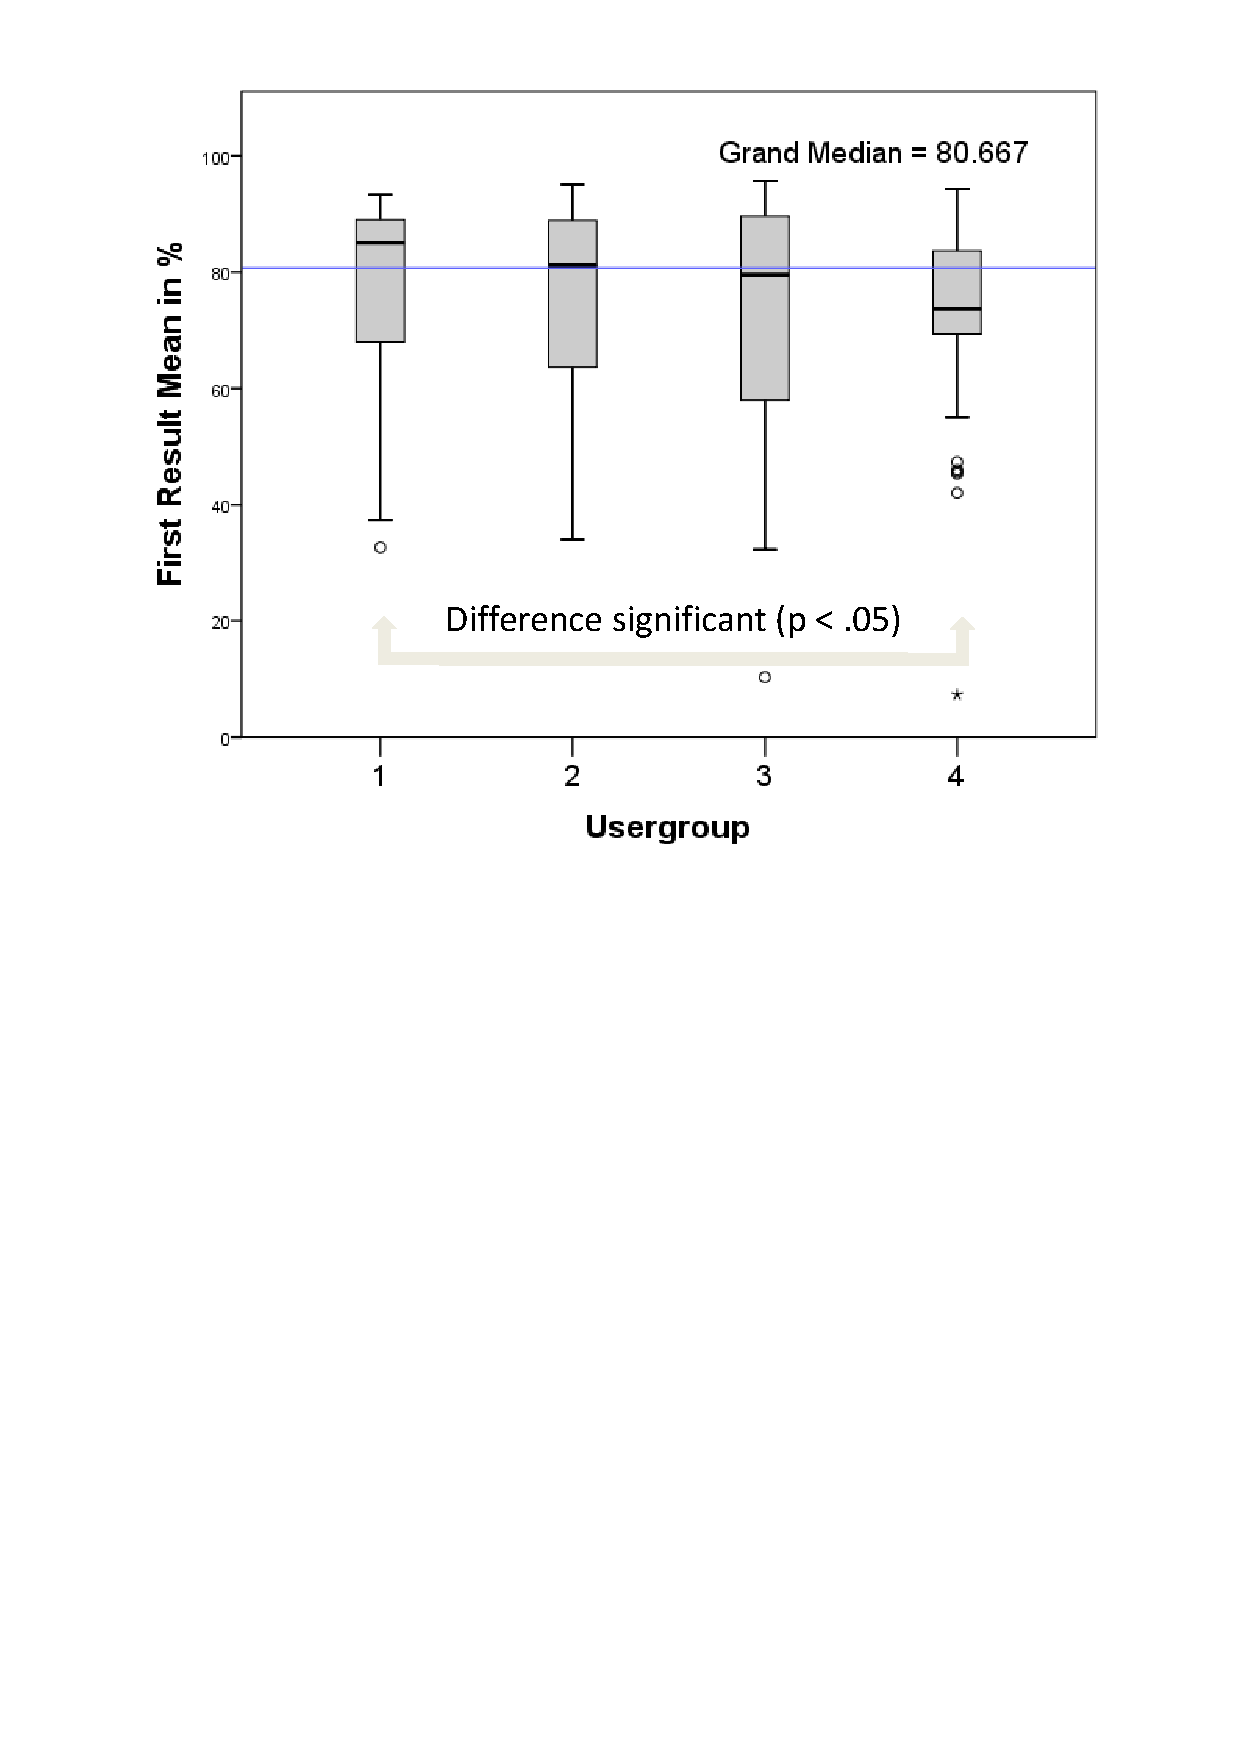
\includegraphics[height = 0.5\textwidth]{NPFirstResultBoxplot.pdf}
%  \caption{Boxplot for FirstResult with Grand Median}
%    \label{fig:NPFirstResultBoxplot} 
%\end{center}
%\end{figure}

\subsection{Tests of dependent samples: \textit{Round}}
A related-Samples Friedman's Two-Way Analysis of Variance by Ranks test \citep{Friedman1937} is applied to compare the values in-between \textit{Rounds}. The null and alternative hypotheses are defined in the following way:

\textbf{Friedman's Test} \\ 
\textbf{H\textsubscript{0}:} \textit{The distributions of the dependent variables are the same across rounds.}\\
\textbf{H\textsubscript{A}:} \textit{At least one distribution is different.}

Friedman's Test results are shown in Table \ref{NPTest} and reject the null hypothesis for all dependent variables. The applied filter does not have an influence on the findings.

\subsection{Implications for parameter estimations}
The findings for the \ac{NP}s underline the magnitude of the statistical noise in the unfiltered data. According to the Kruskal-Wallis-Test, no influence is detectable by \textit{NumberOfColours} when no filter is used. As a result, we only use Filter 1 and Filter 2 for the parameter estimation.\\
Furthermore, not every dependent variable seems to be influenced by the independent variables for the filtered data, so the parameter estimations for those variables might be non-significant.
\newpage
%% ===============================
\section{\acf{LMM}}
\label{ch:Evaluation:sec:LMM}
%% ===============================

%The results from the \ac{LMM} and the \ac{NP}s do not confirm the majority of the hypothesis. In fact, the findings have not confirmed an influence of \textit{Round} and \textit{NumberOfColours}, so one would assume that providing parameter estimates will not introduce further significant findings as well.\\
For the purposes of testing the proposed polynomial relationship between the dependent variables and the \textit{NumberOfColours} as well as the logarithmic influence of \textit{Round}, we examine the data using a \acl{LMM}. This model is a powerful modelling tool that allows the analysis of complex datasets with hierarchical structures \citep{Galecki2013}. As a result, the \acl{LMM} is an appropriate choice with a high power-efficiency for the conditions of our research.

The term \textit{Mixed Model} refers to the use of both fixed and random effects in the same analysis \citep{Seltman2012}. Whereas fixed effects are essential to evaluate the potential polynomial relationship between the independent and dependent variables, random effects aggregate the influences which are not relevant for the purposes of this study. \\ 
Fixed effects are usually related to treatments (\textit{NumberOfColours} and \textit{Trial}), whereas subject effects are defined as random effects (\textit{User}).\\
Subject effects include the individual characteristics of each participant. These effects (e.g. experience with similar tasks or the general ability to perform well in the given task), have an influence on the result and time variables, but are not the focus of our research. As described in Section \ref{ch:Experiment:sec:OnlineImplementation}, one implication for cognitive load experiments on \acf{AMT} is the lack of control over what participants are doing during the experiment. By taking into account these individual influences, and separating them from the focus of the research, the noise of the data can be reduced and can return more significant results.

\paragraph{Normality Assumption}
\ac{LMM} imply the assumption that the data is normally distributed. Yet, the normality assumption is not met by the original data, so a data transformation is necessary.\\
We use the Box-Cox transformation\footnote{Refer to Appendix \ref{Appendix-Formulas} for the formula.} \citep{Sakia1992} that applies a shifted power transformation to adjust the standard deviation and the mean to the requested values for the normal distribution. Since the method is using a range of power transformations, the efficiency of normalizing and variance equalizing for both positively- and negatively-skewed variables can be improved \citep{Osborne2010}. In order to find the optimal input parameter $\lambda$ for the transformation, we implement Osborne's SPSS algorithm. \\
We find suitable $\lambda$-values for the variables \textit{FirstTime} and \textit{DecisionTime}. Nevertheless, no adequate values can be found for all result types, namely \textit{BestTime}, \textit{FinalTime} and \textit{DecisionNumber}.
Figure \ref{fig:SkewKurtosis} provides an explanation for the lack of appropriate $\lambda$-values in the \textit{FirstResult}. No $\lambda$-values can be found that reduce the skewness and kurtosis of the transformed data to a limit at which one can assume a normal distribution. Similar results are returned for \textit{BestResult}, \textit{FinalResult}, \textit{BestTime} and \textit{FinalTime}.
\begin{figure}[htbp] % Transformation	
\begin{center} 
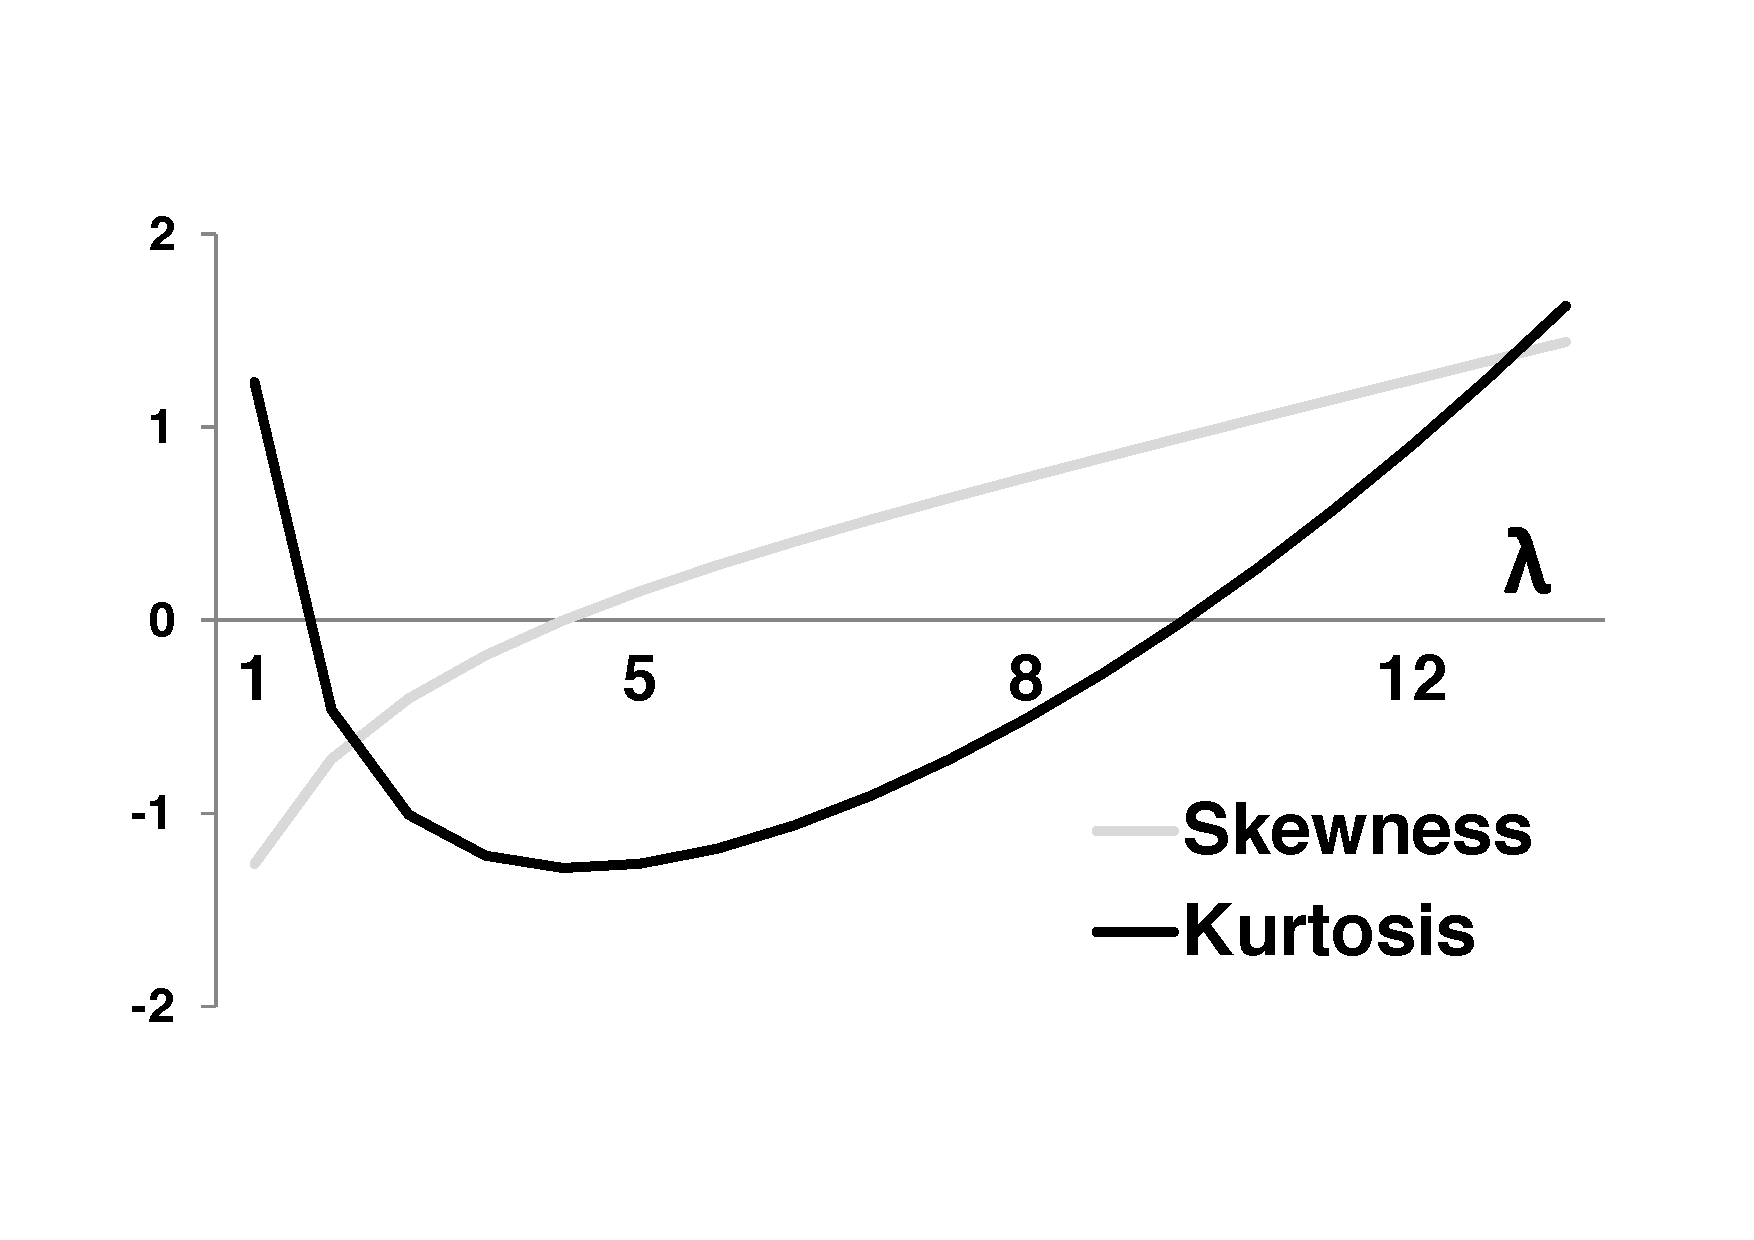
\includegraphics[height = 0.30\textwidth]{SkewKurtosis.pdf}
  \caption{Transformation \textit{FirstResult} - Skewness and Kurtosis for different $\lambda$ values}
    \label{fig:SkewKurtosis} 
\end{center}
\end{figure}
In addition, a test of Normality proves our previous findings that a Box-Cox-transformation is only suitable for \textit{FirstTime} and \textit{DecisionTime}. Since we have a data set smaller than 2000 elements, the Shapiro-Wilk test \citep{Shapiro1965} is used to test the null hypothesis which states that the observed population does not come from a normal distribution. The p-value is greater than 0.05 only for \textit{FirstTime} and \textit{DecisionTime}, so we must retain the null hypothesis for all other variables and conclude that only the data transformation of \textit{FirstTime} and \textit{DecisionTime} comes from a normal distribution.

%\textbf{2. Constant covariance matrix: \makebox[0pt][l]{$\square$}\raisebox{.15ex}{\hspace{0.1em}{\color{red}x}}}\\
%The Box's M test statistic \citep{Box1949} conducted on SPSS tests the null hypothesis that the observed covariance matrices of the dependent variables are not equal across groups. The significance value of the test is less than .10, suggesting that the assumptions are not met and the covariance matrix does differ across usergroups.\\
%\textbf{3. Equal Error variance: \makebox[0pt][l]{$\square$}\raisebox{.15ex}{\hspace{0.1em}{\color{green}$\checkmark$}}}\\ 
%The \cite{Levene1960}'s Test of Equality of Error Variances tests the null hypothesis that the error variance of the dependent variable is not equal across groups.
%The test shows no significant value for the majority of the variables on the .10 significance level and is not significant on the .05 level for two variables. As a result, the null hypothesis can be rejected and we can assume that the equal variances assumption is not violated for each variable.
\paragraph{Conclusion}
The validity of the results based on the \ac{LMM} depends on whether or not its conditions are met \citep{Siegel1957}. Since the normality assumption is not fulfilled for the majority of the variables, the addressed power of the \ac{LMM} might be diluted. \\
According to \cite{Graybill1976}, we can either ignore the violation of the assumptions and proceed with the analysis as if all assumptions were satisfied, or we can use a distribution-free procedure. \\
A distribution-free procedure in the form of non-parametric tests is used in Section \ref{ch:Evaluation:sec:Non-parametrictest}. Yet, these tests do not give information about potential parameter estimations for an implemented model.
Therefore, we continue analysing the data using the \ac{LMM}.

\subsection{Choice of a \ac{LMM} model}
In order to specify a mixed model, several steps, each of which requires an informed decision \citep{Seltman2012}, are necessary. \\
First, the identification of  fixed effects requires the specification of which influences affect the average performances for all individuals.  We assume that the level of \textit{NumberOfColours} and the \textit{Round} number affects each participant.
The \acl{NP} in Section \ref{ch:Evaluation:sec:Non-parametrictest} do not show any significant influence on the population mean from the \textit{Trial}, so we do not take this variable into account as a fixed effect.\\
\begin{figure}[htbp] % RandomIntercept	
\begin{center} 
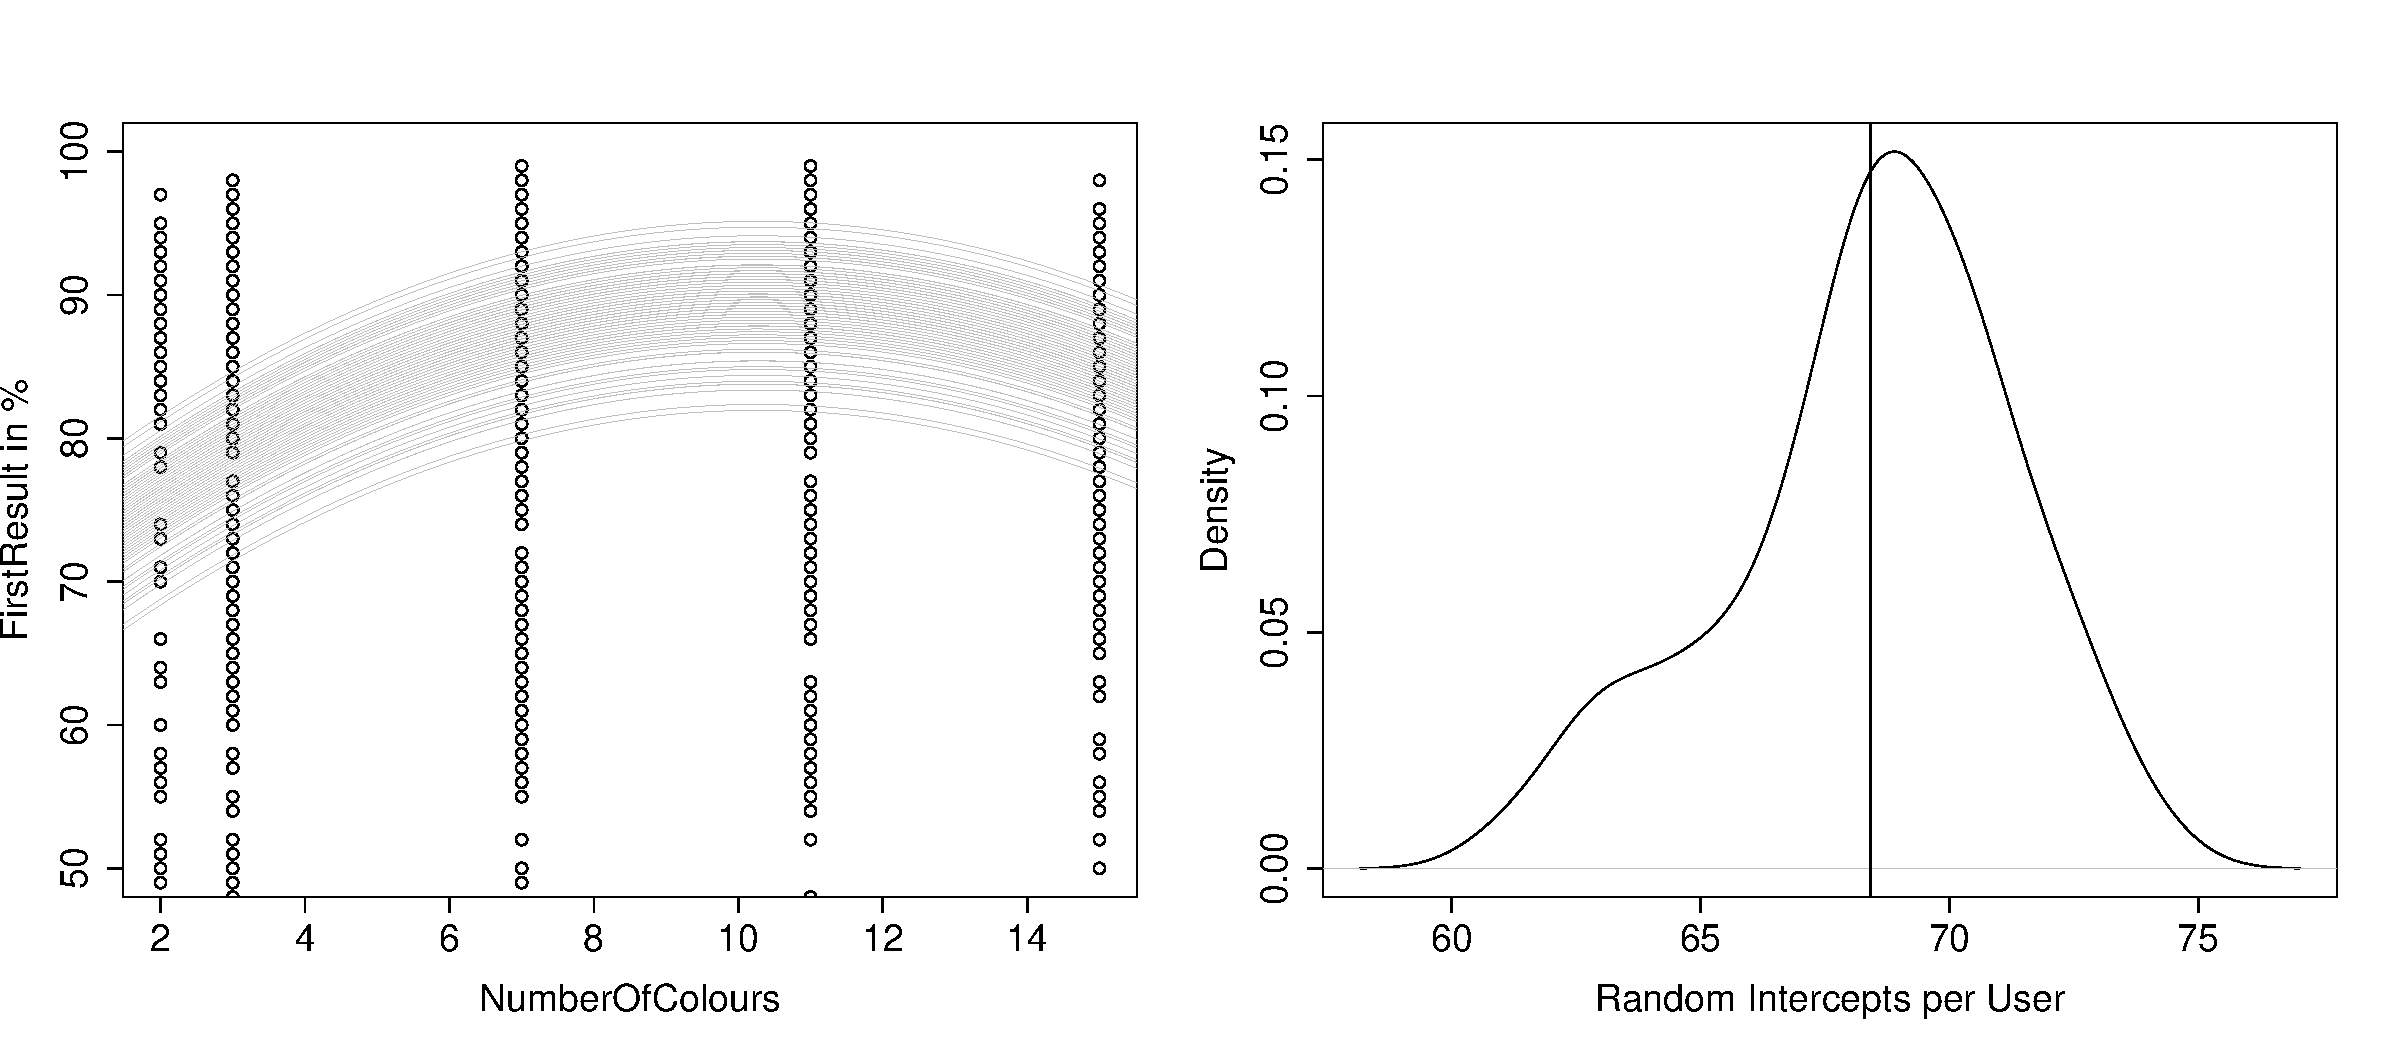
\includegraphics[width = 1\textwidth]{PlotIntercept.pdf}
%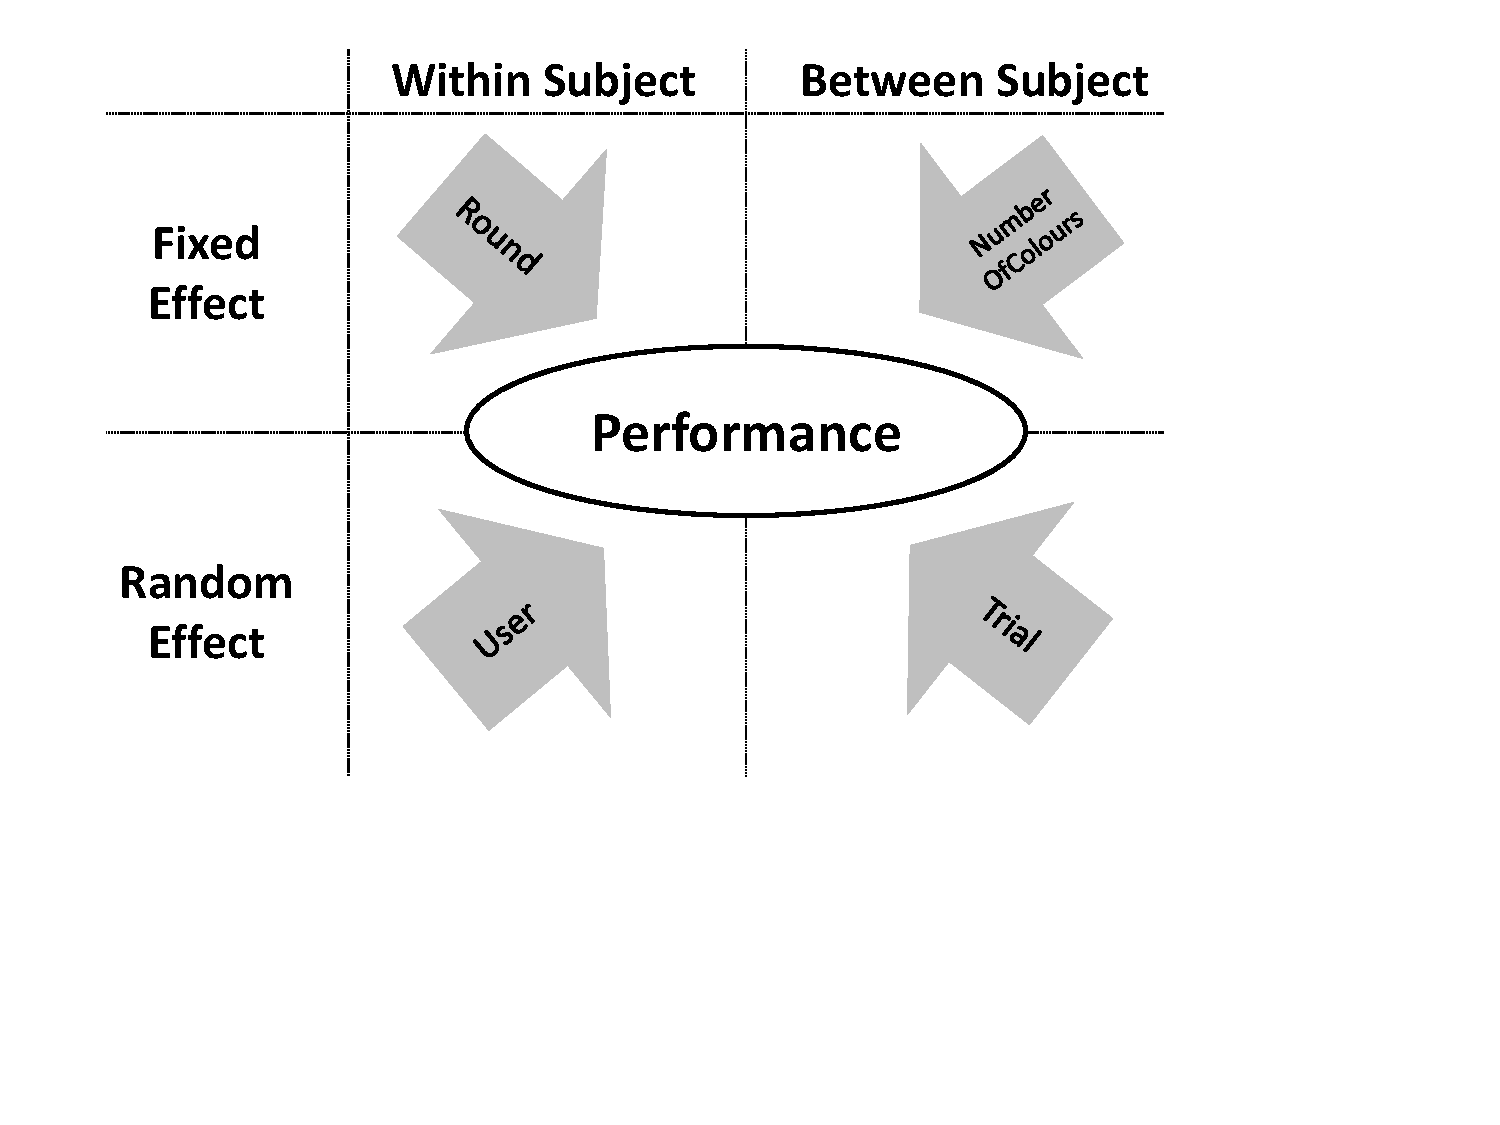
\includegraphics[height = 0.4\textwidth]{UserInfluence.pdf}
  \caption{User-individual Intercepts for the \textit{FirstResult}-parameters}
    \label{fig:Intercepts} 
\end{center}
\end{figure}
Second, we must determine whether the fixed effects are sufficient without a corresponding random effect. We assume that the performance is dependent on the individual characteristics of the participant. In other words, participants have a relatively equal sensitivity to \textit{NumberOfColours} and \textit{Round}, but perform on different levels due to the individual characteristics of each participant. Consequently, every participant has his or her own regression line, with a personalized intercept and an equal slope (Figure \ref{fig:Intercepts}). Due to the lack of influence by the \textit{Trial}, a nested classification of the random intercept is not necessary that would require a combination of \textit{Trial} and \textit{User} for the random intercept.\\
%To display these assumptions in a \ac{LMM}, we use a nested classification of the random intercept. A first random intercept covers the effects of the \textit{Trial} affiliation on the individual participant. Nested within the trial, a second random intercept is introduced to take into account the effects by the individual characteristics.\\
%The nested classification requires the participants to be bi-uniquely assigned to one trial and one usergroup \citep{Galecki2013}. By checking the \ac{AMT}-Worker ID, those participants who played both trials can be identified. Only 5 \ac{AMT}-Users were found, so the  bi-unique relation between user and trial can be assumed. Furthermore, we have excluded participants with the same IP address so that participants who played the game again and again were excluded and one participants consequently only played with one usergroup.\\
Third, correlations among repeated measurements must be taken into account. We assume that all rounds a user plays are equally correlated with each other and the total variation per round, $\sigma^{2} = \sigma^{2}_{\gamma} + \sigma^{2}_{\varepsilon}$, can be partitioned into the "shared" (user) component, $\sigma^{2}_{\gamma}$ and the "unshared" (round) component, $\sigma^{2}_{\varepsilon}$. \\
The \textit{Compound symmetry covariance matrix} is defined as:
\begin{equation}
\begin{split}
{\rm cov}(Y_{ij}, Y_{ik}) = \sigma^{2}_{\gamma} + \sigma^{2}_{\varepsilon} \cdot \mathcal{I}(k = j) \quad \quad \\
Y_{ij}:= Total\;Variance\;of\;User\;i\;in\;Round\;j
\end{split}
\end{equation}
Equation \ref{eq:LMM} shows the used single-level \ac{LMM} with random intercepts.

\fbox{%
\begin{minipage}{6 in}
\begin{equation}
\begin{split}
\label{eq:LMM}
DependentVariable_{i,j} = \quad\quad\quad\quad\quad\quad\quad\quad\quad\quad\quad\quad\quad\quad\quad\quad\quad\quad\quad\quad\quad\quad\quad\quad\quad\\
\boldsymbol{const} \quad\quad\quad\quad\quad\quad\quad\quad\quad\quad\quad\quad\quad\quad
\quad\quad\quad\quad\quad\quad\quad\quad\\
+ \boldsymbol{\beta_1} * NumberOfColours + \boldsymbol{\beta_2} * (NumberOfColours)^2\\
+ \boldsymbol{\beta_3} * log_{10} (Round) + \boldsymbol{r_{i}}+\epsilon_{i,j}\quad\quad\quad\quad\quad\quad\quad\quad
\end{split}
\end{equation}
    \begin{tabular}{ll}
    \textbf{Indexes} & $\;i := Participant,\;j := Round$  \\
    \textbf{Fixed effect 1} &  $\boldsymbol{\beta_1}$ * NumberOfColours + $\boldsymbol{\beta_2}$ * $(NumberOfColours)^2$\\
    \textbf{Fixed effect 2} &  $\boldsymbol{\beta_3} * log_{10}(Round)$\\
    \textbf{Random effect} &  $\boldsymbol{r_i}:=$ Random intercept per User i\\
    \textbf{Error} &  $\epsilon_{i,j}$\\
    \end{tabular}%
\end{minipage}}

\paragraph{Implementation in R}
For the implementation of the \ac{LMM}s we use the \textbf{nlme}-package of the software programming language \textbf{R}\footnote{Refer to \cite{R2012}.} . The package is especially designed for \ac{LMM}s  \citep{Pinheiro2013} and fits a linear mixed-effects model in the formulation described by \cite{Laird1982}.\\
The model described in \ref{eq:LMM} is implemented using the following code:
\begin{verbatim}
> LMM <- lme(DV ~ 1 + NumberOfColours + NumberOfColours2 + RoundL, 
+               random=~1 | User, 
+               correlation=corCompSymm(form = ~ RoundL| User))
\end{verbatim}

\subsection{Results for the \ac{LMM}}

According to the \acl{NP} findings, only the filtered data is considered for the parameter estimations.\\
The results for the fixed effects of the \ac{LMM} can be interpreted in the same way as an ANOVA regression. Nevertheless, we must take into account that the intercept represents the mean over all subjects and each individual subject has its own individual intercept \citep{Seltman2012}. The population made up by all individual intercepts approximately follows a normal distribution, with the computed overall estimate as the mean and the variance of the random intercepts (Figure \ref{fig:Intercepts}).

\paragraph{Filter 1: Users with \textit{BestResult} $\geq$ 80\% for each round}
\textbf{\textit{NumberOfColours} }\\
The \ac{LMM} returns significant results for the \textit{FirstResult}, the \textit{DecisionTime} and the \textit{DecisionNumber}.  Moreover, the parameters of \textit{FirstResult}  and \textit{DecisionTime} are all significant, \textit{DecisionNumber} has significant parameters with the exception of quadratic parameter that is only significant on the 0.1 level. \\
Consequently, the hypothesis that there is an \textbf{$\cap$}-relation between the performance of a participant and the \textit{NumberOfColours} is only supported for the \textit{FirstResult}. In addition, the results for \textit{DecisionTime} and \textit{DecisionNumber} show a quadratic relation with \textit{NumberOfColours}, as expected by the hypothesis. The \textit{DecisionTime} reaches its maximum and the \textit{DecisionNumber} its minimum for a medium level of information granularity. No significant results are signalized for the \textit{First-}, \textit{Best-}, and \textit{FinalTime}.

\afterpage{
\begin{landscape}
\begin{table}
\begin{center}
\begin{tabular}{l D{.}{.}{5.5} @{}D{.}{.}{5.5} @{}D{.}{.}{5.5} @{}D{.}{.}{5.5} @{}D{.}{.}{5.5} @{}D{.}{.}{5.5} @{}D{.}{.}{4.5}@{}D{.}{.}{4.5} @{}}
\toprule
                 & \multicolumn{1}{c}{First} & \multicolumn{1}{c}{Best} & \multicolumn{1}{c}{Final}  
                 & \multicolumn{1}{c}{First} & \multicolumn{1}{c}{Best} & \multicolumn{1}{c}{Final}
                 & \multicolumn{1}{c}{Decision} & \multicolumn{1}{c}{Decision}\\
                 & \multicolumn{1}{c}{Result} & \multicolumn{1}{c}{Result} & \multicolumn{1}{c}{Result} 
                 & \multicolumn{1}{c}{Time} & \multicolumn{1}{c}{Time}& \multicolumn{1}{c}{Time}
                 &\multicolumn{1}{c}{Number}& \multicolumn{1}{c}{Time} \\
\midrule
(Intercept)      & 85.46^{***}  & 89.82^{***}   & 89.40^{***}   & 44.09^{***}  & 53.50^{***}  & 63.38^{***}  & 2.26^{***}   & 28.91^{***} \\
                 & (1.29)       & (0.92)        & (0.97)        & (4.30)       & (4.44)       & (5.23)       & (0.18)        & (2.14)      \\
NumberOfColours  & 0.82^{*}     & 0.41          & 0.43          & 1.83         & 0.84         & 0.31         & 0.13^{**}     & -1.29^{*}   \\
                 & (0.36)       & (0.26)        & (0.27)        & (1.22)       & (1.23)       & (1.49)       & (0.05)        & (0.61)      \\
NumberOfColours2 & -0.05^{**}   & -0.03^{\cdot} & -0.03^{\cdot} & -0.10        & -0.02        & 0.03         & -0.01^{\cdot} & 0.07^{*}    \\
                 & (0.02)       & (0.01)        & (0.02)        & (0.07)       & (0.07)       & (0.09)       & (0.00)       & (0.03)      \\
RoundL           & 2.24^{\cdot} & 2.84^{***}    & 2.99^{***}    & -17.39^{***} & -16.16^{***} & -14.54^{***} & -1.21^{***}   & 4.86^{***}  \\
                 & (1.29)       & (0.76)        & (0.81)        & (3.37)       & (3.27)       & (3.25)       & (0.11)        & (1.40)      \\
\midrule
%Log Likelihood   & -1711.65     & -1470.47      & -1502.79      & -2252.97     & -2245.24     & -2274.95     & -527.98       \\
%$\sigma$: Intercept Trial &    <0.01    &    <0.01     &   <0.01      &  <0.01     &       <0.01 & <0.01 &  <0.01 \\
$\sigma$: Intercept User in Trial &   3.52     &     2.84    &      2.99 &13.62&  12.81     &    17.58   &   0.59  & 7.11 \\
$\sigma$: Residual         &     5.50   &    3.19   &    3.40    &       14.09&   14.72    &    13.45   & 0.47& 5.82\\
\bottomrule
\vspace{-3mm}\\
\multicolumn{9}{l}{\textsuperscript{***}$p<0.001$, 
  \textsuperscript{**}$p<0.01$, 
  \textsuperscript{*}$p<0.05$, 
  \textsuperscript{$\cdot$}$p<0.1$}
\end{tabular}
\caption{LMM-Results for Filter 1}
\label{table:coefficients}
\end{center}
\end{table}
\end{landscape}} 
\begin{figure}[H] % Filter1PlotColoursFirstResult	
\begin{center}
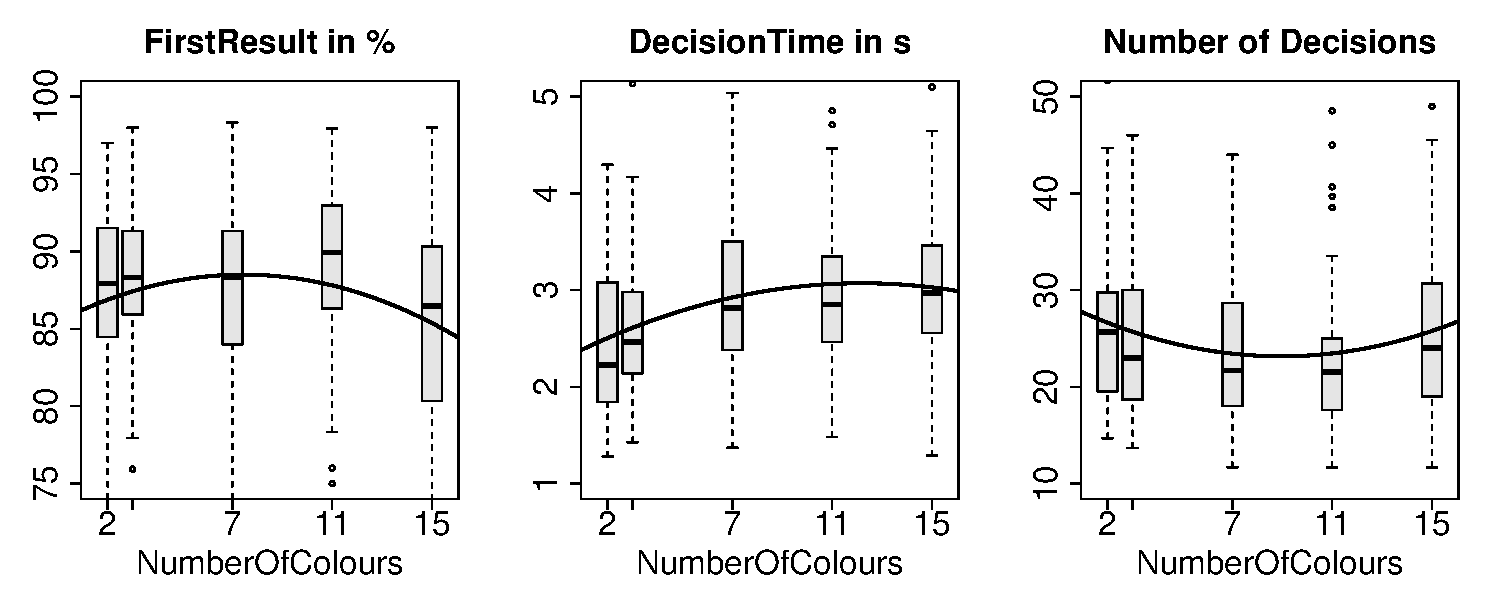
\includegraphics[width = 1\textwidth]{Filter2PlotInformationGranularity.pdf}    
  \caption[Results for Filter 1: Information Granularity]{Results for Filter 1: Information Granularity\footnotemark}
    \label{fig:Results for Filter 1: Information Granularity} 
\end{center}
\end{figure}
\footnotetext{The values for the dependent variables are adjusted so they exclude the predicted effect by \textit{Round}.}

\textbf{\textit{Round} }\\
The learning effect, hence the influence of the \textit{Round}, is significant for all variables. So we can conclude that there is a learning effect when playing several rounds in the experiment, and the slope of this learning effect diminishes with the number of rounds played, as indicated by the logarithmic relation. Surprisingly, the number of decisions increases with the number of rounds, as supposed to the expected decline. \\
Since the time it takes participants to reach the \textit{FinalResult} is represented by the product of \textit{DecisionNumber} and \textit{DecisionTime}, two opposing trends can be identified when describing the round effect on the \textit{FinalTime}. Whereas the number of decisions increases, the time to take a decision decreases. The \ac{LMM} returns a negative parameter for \textit{FinalTime},  indicating that the decrease in the decision times outbalances the increase in the number of decisions.  
\begin{figure}[H] % Filter1PlotColoursFirstResult	
\begin{center}
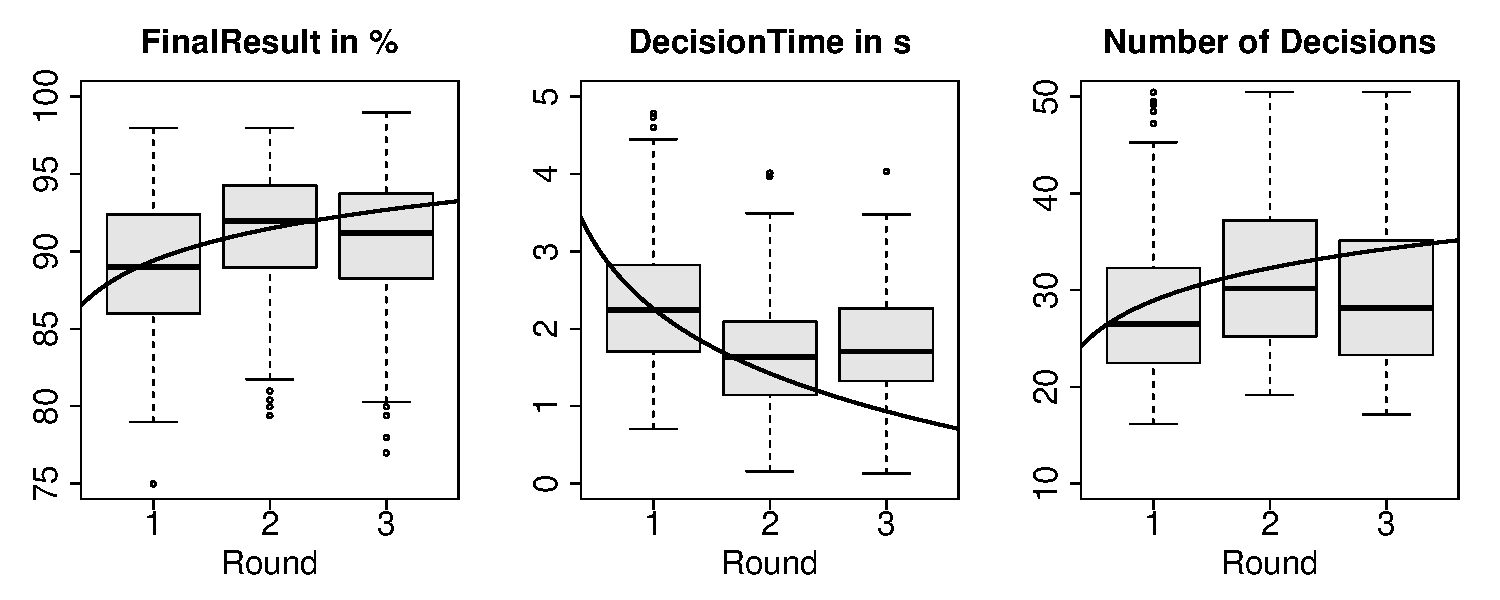
\includegraphics[width = 1\textwidth]{Filter2PlotLearningEffect.pdf}  
  \caption[Results for Filter 1: Learning effect]{Results for Filter 1: Learning effect\footnotemark}
    \label{fig:Results for Filter 1: Learning effect} 
\end{center}
\end{figure}
\footnotetext{The values for the dependent variables are adjusted so they exclude the predicted effect by \textit{NumberOfColours}.}
\textbf{\textit{User} }\\
The standard deviations of the \textit{User} random intercepts are high, and underline the influential magnitude of the individual performance characteristics of the participants. In particular, the \textit{DecisionNumber} and \textit{DecisionTime} seem to be most affected by the individual, since the relative standard deviation is the highest for all variables. 

%
%%\begin{landscape}
%\begin{table}
%\begin{center}
%\begin{tabular}{l D{.}{.}{5.5} @{}D{.}{.}{5.5} @{}D{.}{.}{5.5} @{}D{.}{.}{4.5} @{}D{.}{.}{5.5} @{}}
%\toprule
%                 & \multicolumn{1}{c}{First} & \multicolumn{1}{c}{Best} & \multicolumn{1}{c}{Final} & \multicolumn{1}{c}{Decision} &\multicolumn{1}{c}{Decision}\\
%                 & \multicolumn{1}{c}{Result} & \multicolumn{1}{c}{Result} & \multicolumn{1}{c}{Result} & \multicolumn{1}{c}{Time} &\multicolumn{1}{c}{Number}\\
%\midrule
%(Intercept)      & 85.46^{***}  & 89.82^{***}   & 89.40^{***}   & 2.26^{***}    & 28.91^{***} \\
%                 & (1.29)       & (0.92)        & (0.97)        & (0.18)        & (2.14)      \\
%NumberOfColours  & 0.82^{*}     & 0.41          & 0.43          & 0.13^{**}     & -1.29^{*}   \\
%                 & (0.36)       & (0.26)        & (0.27)        & (0.05)        & (0.61)      \\
%NumberOfColours2 & -0.05^{**}   & -0.03^{\cdot} & -0.03^{\cdot} & -0.01^{\cdot} & 0.07^{*}    \\
%                 & (0.02)       & (0.01)        & (0.02)        & (0.00)        & (0.03)      \\
%RoundL           & 2.24^{\cdot} & 2.84^{***}    & 2.99^{***}    & -1.21^{***}   & 4.86^{***}  \\
%                 & (1.29)       & (0.76)        & (0.81)        & (0.11)        & (1.40)      \\
%\midrule
%%AIC              & 3439.31      & 2956.94       & 3021.57       & 1071.96       & 3677.81     \\
%%BIC              & 3473.31      & 2990.94       & 3055.57       & 1105.96       & 3711.81     \\
%%Log Likelihood   & -1711.65     & -1470.47      & -1502.79      & -527.98       & -1830.91    \\
%%$\sigma$: Intercept Trial &    <0.01    &    <0.01     &   <0.01      &  <0.01     &       <0.01\\
%$\sigma$: Intercept User &   3.52     &     2.84    &      2.99 &   0.59  & 7.11 \\
%$\sigma$: Residual         &     5.50   &    3.19   &    3.40    &       0.47 & 5.82\\
%\bottomrule
%\vspace{-3mm}\\
%\multicolumn{6}{l}{\textsuperscript{***}$p<0.001$, 
%  \textsuperscript{**}$p<0.01$, 
%  \textsuperscript{*}$p<0.05$, 
%  \textsuperscript{$\cdot$}$p<0.1$}
%\end{tabular}
%\caption{LMM-Results for Filter 1}
%\label{table:coefficients}
%\end{center}
%\end{table}
%%\end{landscape}

\paragraph{Filter 2: Filter 1 + \textit{NumberOfColours} $\geq$ 7}
\textbf{\textit{NumberOfColours} }\\
When only including the treatment groups that were assigned to 7, 11 and 15 colours, the parameter estimations become significant for \textit{FirstResult}, \textit{BestResult} and \textit{FinalResult}. The \textbf{$\cap$}-relation with \textit{NumberOfColours} is consequently confirmed when looking at this range of \textit{NumberOfColours}. These findings, however, do not support our hypothesis that the performance will be best on a medium information granularity, since a peak can be found for the 11-colours treatment. In addition, none of the previous findings for \textit{DecisionNumber} and \textit{DecisionTime} are confirmed in Filter 2.

\textbf{\textit{Round} }\\
 A learning effect can also be detected for this data set, with an exception of \textit{FirstResult} - the \ac{LMM} does not return significant results for its parameters. 

\textbf{\textit{User} }\\
The standard deviation for the \textit{User} random intercepts again show high values yet again, so the impact of excluding the variance caused by individual characteristics is underlined.\\

\begin{figure}[H] % Filter1PlotColoursFirstResult	
\begin{center}
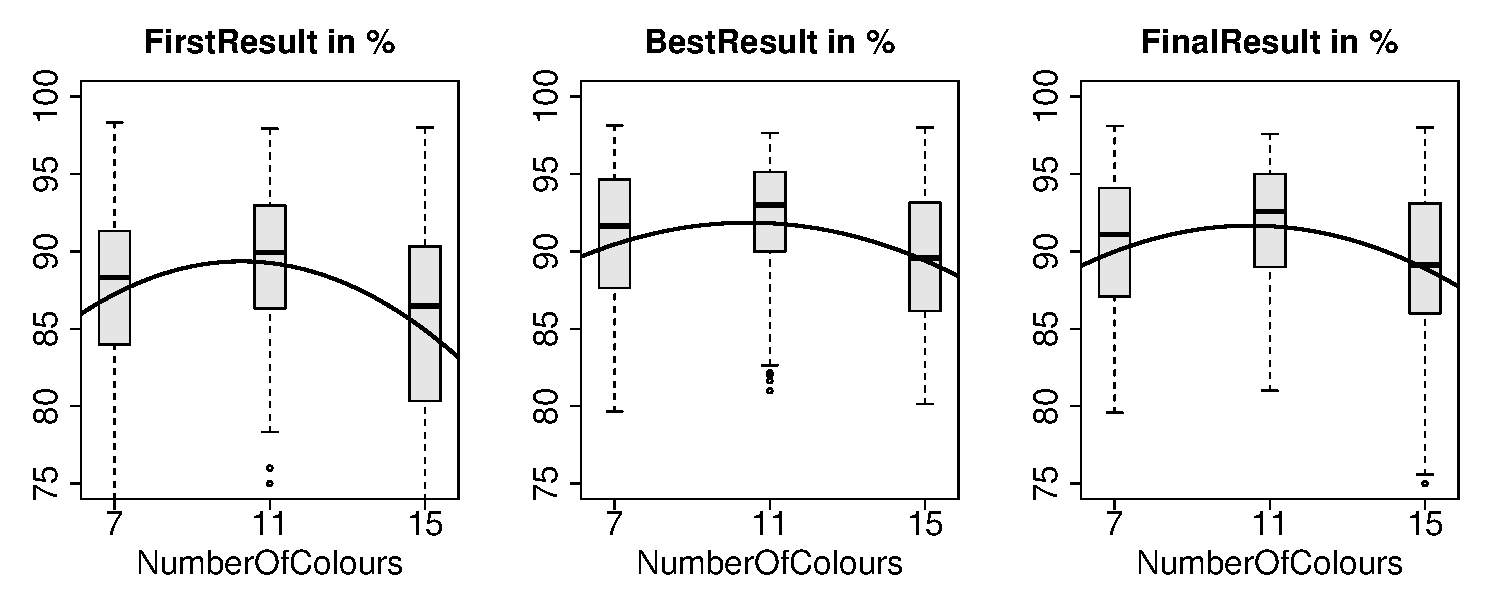
\includegraphics[width = 1\textwidth]{Filter3PlotInformationGranularity.pdf}    
  \caption[Results for Filter 2: Information Granularity]{Results for Filter 2: Information Granularity\footnotemark}
    \label{fig:Results for Filter 3: Information Granularity} 
\end{center}
\end{figure}
\footnotetext{The values for the dependent variables are adjusted so they exclude the predicted effect by \textit{Round}.}

%\afterpage{
%\begin{landscape}
%\begin{table}
%\begin{center}
%\begin{tabular}{l D{.}{.}{5.5} @{}D{.}{.}{4.5} @{}D{.}{.}{4.5} @{}D{.}{.}{5.5} @{}D{.}{.}{5.5} @{}D{.}{.}{5.5} @{}D{.}{.}{4.5} @{}}
%\toprule
%                 & \multicolumn{1}{c}{FirstResult} & \multicolumn{1}{c}{BestResult} & \multicolumn{1}{c}{FinalResult} & \multicolumn{1}{c}{FirstTime} & \multicolumn{1}{c}{BestTime} & \multicolumn{1}{c}{FinalTime} & \multicolumn{1}{c}{DecisionTime} \\
%\midrule
%(Intercept)      & 68.41^{***} & 78.95^{***} & 76.55^{***} & 54.92^{*}    & 84.20^{***} & 102.08^{***} & 3.34^{***}  \\
%                 & (6.87)      & (5.13)      & (5.34)      & (22.90)      & (22.49)     & (26.06)      & (0.94)      \\
%NumberOfColours  & 4.08^{**}   & 2.47^{*}    & 2.88^{**}   & -0.25        & -5.34       & -7.31        & -0.07       \\
%                 & (1.36)      & (1.01)      & (1.05)      & (4.52)       & (4.44)      & (5.15)       & (0.19)      \\
%NumberOfColours2 & -0.20^{**}  & -0.12^{*}   & -0.14^{**}  & 0.00         & 0.26        & 0.36         & 0.00        \\
%                 & (0.06)      & (0.05)      & (0.05)      & (0.21)       & (0.20)      & (0.23)       & (0.01)      \\
%RoundL           & 2.26        & 3.73^{***}  & 3.64^{***}  & -18.79^{***} & -12.15^{**} & -11.47^{**}  & -1.31^{***} \\
%                 & (1.43)      & (0.96)      & (1.03)      & (4.32)       & (4.25)      & (4.03)       & (0.15)      \\
%\midrule
%Log Likelihood   & -1059.20    & -940.58     & -960.30     & -1429.44     & -1423.93    & -1427.96     & -351.77     \\
%$\sigma$: Intercept Trial &    <0.01    &    <0.01     &   <0.01      &  <0.01     &       <0.01 & <0.01 &  <0.01 \\
%$\sigma$: Intercept User in Trial &    4.16    &   3.22      &     3.31    &      14.35 &     14.09  & 16.87 & 0.61  \\
%$\sigma$: Residual         &    4.77    &     3.17    &    3.43    &    14.25   &   14.02    &     13.32  & 0.49\\
%\bottomrule
%\vspace{-3mm}\\
%\multicolumn{8}{l}{\textsuperscript{***}$p<0.001$, 
%  \textsuperscript{**}$p<0.01$, 
%  \textsuperscript{*}$p<0.05$, 
%  \textsuperscript{$\cdot$}$p<0.1$}
%\end{tabular}
%\caption{LMM-Results for Filter 2}
%\label{table:Filter2Results}
%\end{center}
%\end{table}
%\end{landscape}}


\begin{table}
\begin{center}
\begin{tabular}{l D{.}{.}{5.5} @{}D{.}{.}{4.5} @{}D{.}{.}{4.5} @{}D{.}{.}{5.5} @{}D{.}{.}{5.5} @{}D{.}{.}{5.5} @{}D{.}{.}{4.5} @{}}
\toprule
                 & \multicolumn{1}{c}{First} & \multicolumn{1}{c}{Best} & \multicolumn{1}{c}{Final} & \multicolumn{1}{c}{Decision} &\multicolumn{1}{c}{Decision}\\
                 & \multicolumn{1}{c}{Result} & \multicolumn{1}{c}{Result} & \multicolumn{1}{c}{Result} & \multicolumn{1}{c}{Time} &\multicolumn{1}{c}{Number}\\
\midrule
(Intercept)      & 68.41^{***} & 78.95^{***} & 76.55^{***} & 3.34^{***}  & 36.34^{***} \\
                 & (6.87)      & (5.13)      & (5.34)      & (0.94)      & (10.85)     \\
NumberOfColours  & 4.08^{**}   & 2.47^{*}    & 2.88^{**}   & -0.07       & -2.78       \\
                 & (1.36)      & (1.01)      & (1.05)      & (0.19)      & (2.14)      \\
NumberOfColours2 & -0.20^{**}  & -0.12^{*}   & -0.14^{**}  & 0.00        & 0.14        \\
                 & (0.06)      & (0.05)      & (0.05)      & (0.01)      & (0.10)      \\
RoundL           & 2.26        & 3.73^{***}  & 3.64^{***}  & -1.31^{***} & 6.26^{***}  \\
                 & (1.43)      & (0.96)      & (1.03)      & (0.15)      & (1.63)      \\
\midrule
AIC              & 2134.39     & 1897.16     & 1936.59     & 719.54      & 2288.81     \\
BIC              & 2164.69     & 1927.46     & 1966.89     & 749.84      & 2319.11     \\
Log Likelihood   & -1059.20    & -940.58     & -960.30     & -351.77     & -1136.41    \\
%$\sigma$: Intercept Trial &    <0.01    &    <0.01     &   <0.01      &  <0.01     &       <0.01 \\
$\sigma$: Intercept User&    4.16    &   3.22      &     3.31    & 0.61  & 7.10\\
$\sigma$: Residual         &    4.77    &     3.17    &    3.43    & 0.49 & 5.33\\
\bottomrule
\vspace{-3mm}\\
\multicolumn{6}{l}{\textsuperscript{***}$p<0.001$, 
  \textsuperscript{**}$p<0.01$, 
  \textsuperscript{*}$p<0.05$, 
  \textsuperscript{$\cdot$}$p<0.1$}
\end{tabular}
\caption{LMM-Results for Filter 2}
\label{table:Filter2Results}
\end{center}
\end{table}


\begin{table}[htbp] % Usergroup and Hypotheses
  \centering
  \caption{Overview: Accepted and Rejected Hypotheses}
  \label{tab:HypothesesEvalutation}
    \begin{tabular}{cc|rrr}
    \toprule
    \textbf{Treatment} & \textbf{\# Colours} & \multicolumn{3}{c}{\textbf{Hypotheses}} \\
    \midrule
    \textbf{1} & 2     &  & \multicolumn{1}{l}{H1a-c: } & \multicolumn{1}{l}{Treatment 1+2 < 3 > 4+5} \\
    \textbf{2} & 3     &       & \multicolumn{1}{l}{H2: } & \multicolumn{1}{l}{Treatment 1+2 < 3 > 4+5} \\
    \textbf{3} & 7    &    &  \multicolumn{1}{l}{H3: } & \multicolumn{1}{l}{Treatment 1+2 > 3 < 4+5} \\
    \textbf{4} & 11    &    &  \multicolumn{1}{l}{H4a-c: } & \multicolumn{1}{l}{Round 1 < 2 < 3} \\
    \textbf{5} &  15	   &    &  \multicolumn{1}{l}{H5: } & \multicolumn{1}{l}{Round 1 > 2 > 3} \\
     & 		&    &  \multicolumn{1}{l}{H6: } & \multicolumn{1}{l}{Round 1 > 2 > 3} \\
     & 		&    &  \multicolumn{1}{l}{H7a-c: } & \multicolumn{1}{l}{Round 1 > 2 > 3} \\
    \bottomrule
    \end{tabular}%
\end{table}%

%%% ===============================
%\section{Hypotheses Test}
%\label{ch:Evaluation:sec:HypothesesTest}
%%% ===============================
%
%For all hypotheses, we define the null hypothesis as a point hypothesis, which states that the means for all treatments are the same. The alternative hypotheses can be expressed by saying: "at least one of the treatment means differ from all the others".
%\begin{equation}
%\begin{split}
%NumberOfColours: \mu_1=\dots=\mu_4  \\
%Round: \mu_1=\dots=\mu_3 \\
%\mu_i = mean \quad
%\end{split}
%\end{equation}
%
%that all means for the outcome variables the variable \textit{number of colours} has no significant influence on the outcome variables FirstResult, BestResult, FinalResult and DecisionTime.
%
%Linear transformation Number of COlours 4x+3
%The extracted data is used to test the hypothesis introduced in Section \ref{ch:Literature Review:sec:Hypotheses}.
%
%\begin{table}[htbp] % Usergroup and Hypotheses
%  \centering
%  \caption{Usergroups and Nullhypotheses}
%  \label{tab:NullHypotheses}
%    \begin{tabular}{cc|rrr}
%    \toprule
%    \textbf{Usergroup} & \textbf{\# Colours} & \multicolumn{3}{c}{\textbf{Null Hypotheses}} \\
%    \midrule
%    \textbf{1} & 3     & \textbf{} & \multicolumn{1}{l}{H1a-c: } & \multicolumn{1}{l}{   $\mu_1=\dots=\mu_4$ } \\
%    \textbf{2} & 7     &       & \multicolumn{1}{l}{H2} & \multicolumn{1}{l}{Usergroup 2+3 > 1+4} \\
%    \textbf{3} & 11    &       & \multicolumn{1}{l}{H3a-c: } & \multicolumn{1}{l}{Round 1 < 2 < 3} \\
%    \textbf{4} & 15    & \textbf{} & \multicolumn{1}{l}{H4} & \multicolumn{1}{l}{Round 1 < 2 < 3} \\
%    \bottomrule
%    \end{tabular}%
%\end{table}%
%
